\documentclass[12pt]{report}

\usepackage[a4paper,bindingoffset=0.2in,%
            left=1.5in,right=1in,top=1in,bottom=1in,%
            footskip=.25in]{geometry}


\usepackage[utf8]{inputenc}
\usepackage[english]{babel}
\pagenumbering{roman}
\usepackage{graphicx} 
\usepackage[labelformat=empty]{subfig}
\usepackage{biblatex}
\usepackage{csquotes} % Biblatex throws warning if not included
\usepackage{amsmath}
\usepackage{amsthm}
\usepackage{setspace} 
\usepackage{amssymb} 
\usepackage{esint} 
\usepackage{cool} % A ridiculous number of macros for complex symbols
\usepackage{booktabs,makecell} % specifically for the table of std

% specific external file paths
\addbibresource{refs.bib}
\graphicspath{ {./graphics/} }



\newtheorem{theorem}{Theorem}[section]
%\def\thetheorem{\unskip}
\newtheorem{proposition}[theorem]{Proposition}
%\def\theproposition{\unskip}
\newtheorem{conjecture}[theorem]{Conjecture}
\def\theconjecture{\unskip}
\newtheorem{corollary}[theorem]{Corollary}
\newtheorem{lemma}[theorem]{Lemma}
\newtheorem{observation}[theorem]{Observation}
%\def\thelemma{\unskip}
\newtheorem{definition}{Definition}
\numberwithin{definition}{section}
%\def\thedefinition{\unskip}
\newtheorem{remark}{Remark}
\def\theremark{\unskip}
\newtheorem{question}{Question}
\def\thequestion{\unskip}
\newtheorem{example}{Example}
\def\theexample{\unskip}
\newtheorem{problem}{Problem}
\newtheorem{exercise}[theorem]{Exercise}


% Various rules for hiding environments

\newif\ifhideproofs
% \hideproofstrue %uncomment to hide proofs

\ifhideproofs
\usepackage{environ}
\NewEnviron{hide}{}
\let\proof\hide
\let\endproof\endhide
\fi

% notes environ

\newif\ifhidetodos

% \hidetodostrue %uncomment to disable todos package

\ifhidetodos
\usepackage[disable]{todonotes}
\else
\usepackage{todonotes}
\fi


\begin{document}

  \doublespacing
  
\begin{titlepage}

   \begin{center}
      

      The Pólya–Szegő Conjecture on Polygons: A Numerical Approach

            
     
       By
              


      LOGAN REED

     
            
        A thesis submitted to the \\
       Graduate School–Camden\\
       Rutgers, The State University of New Jersey\\
       In partial fulfullment of the requirements\\
       For the degree of Master of Science\\
       Graduate Program in Mathematical Sciences \\
       Written under the direction of \\
       Siqi Fu\\
       And approved by \\
       \noindent\rule{4cm}{0.4pt}\\
       Dr. Siqi Fu\\
      \noindent\rule{4cm}{0.4pt}\\
       Dr. Haydee Herrera-Guzman\\
           \noindent\rule{4cm}{0.4pt}\\
       Dr. Haisheng Li\\

         \vspace{0.8cm}
       Camden, New Jersey\\
       May 2023
            
       \vspace{0.8cm}
     
  
        
            
   \end{center}
   
\end{titlepage}





  \begin{center}

\break
  THESIS ABSTRACT\\
 
      The Pólya–Szegő Conjecture on Polygons: A Numerical Approach \\
         by LOGAN REED\\
     
     Thesis Director: \\
     Siqi Fu
  \end {center}

  In this thesis
  we introduce a numerical approach adapted to the minimization of the first eigenvalue of the Laplacian with respect to the Dirichlet boundary condition on a polygonal domain of fixed area.
  We utilize the method of fundamental solutions and a standard descent method to optimize the first eigenvalue with respect to the vertices of the domain.
  This algorithm enables us to study the validity of the Pólya-Szegő conjecture for polygons with five or more sides, which has remained open since $1950$.
  We also prove some properties of the Dirichlet eigenvalues when we have a polygonal domain.


  
\break





\tableofcontents


\newcommand{\comment}[1]{}


\break


\pagenumbering{arabic}
\pagestyle{myheadings}



\chapter{Introduction}

\break
\section {Physical Motivation}


Physical drums consist of a rigid shell with a membrane which produces sound when hit.
A similar thing can be ``created'' in a pure mathematical setting by studing specific partial differential equations over a closed region.
Specifically, the frequencies of the drum membrane corresponds to the eigenvalues of the Dirichlet Laplacian.
This construction makes it possible to ``hear'' drums where the shape of the drumhead is any closed and simple curve.
To do this, we begin with the shape of our drumhead, which is a region of the real plane bounded by piecewise smooth curves.
Since we wish to emulate the physical properties of a drum, we want to define some system that models the vibration of the drum membrane which produces the sound.
This is done using the wave equation to model the vertical displacement of the membrane over our domain, with no displacement of the membrane on the boundary.
The system ends up being equivalent to solving the Dirichlet Laplacian, and we use this fact to connect the eigenvalues with the fundamental frequencies and overtones of the drum.
Thus, by modeling the vibration of the drumhead using the Dirichlet Laplacian and studying its properties, we can ``hear'' sound via the eigenvalues.
Let us show this construction in more detail.


Consider a homogeneous elastic drumhead, or membrane, stretched over a rigid frame.
We will represent the frame as a domain $\Omega \subset \mathbb{R}^{2}$.
Take the function $u(x,y,t)$ to be the vertical displacement of the membrane from its resting position.
Then for any disk $D \subset \Omega$, Newton's second law of motion implies that
$$ \int_{\partial D} T \frac{\partial u}{\partial \textbf{n}} \, dS = \int_{ D} \rho u_{tt} \, dA $$
where $T$ is the constant tension, $\rho$ is the density constant, and $\textbf{n}$ is the outward normal of the boundary.
By the divergence theorem, we have
$$ \int_{D} T \Delta u \, dA = \int_{D} \rho u_{tt} \, dA $$
where $\Delta$ is the Laplace operator.
From this we can get the wave equation on $\Omega$
$$ u_{tt} = c^{2} \Delta u $$
where we define $u$ to be $0$ on the boundary and where $c = \sqrt{T / \rho}$.
We can solve this wave equation using $u(x,y,t) = T(t)V(x,y)$ which gives us
$$ \frac{T''}{c^{2}T} = \frac{\Delta V}{V} = - \lambda $$
and finally we have reduced our problem to the Dirichlet Laplacian
$$ \Delta V = - \lambda V $$
where $V$ on the boundary is zero.

\break


\section{Background}
The classical isoperimetric problem is as follows: Among all plane figures with a given perimeter $L$, which one encloses the greatest area $A$?
In other words, among all plane figures with a given area, which one has the least perimeter?
The importance of the isoperimetric problem can hardly be understated.
One can find it in Vergil's version of the legend of Dido as well as one of the fundamental problems in the classical calculus of variations.
As far back as $200$BC, a greek mathematician named Zenodorus showed that a circle has greater area than any polygon with the same perimeter (see \cite{pappus}).
Zenodorus also proved that for regular $n $-polygons with the same perimeter $L$, its area $A_{n}$ increases as $n \to \infty$, and that $A_{n} \leq \frac{L^{2}}{4\pi}$.

In 1877, Lord Rayleigh famously conjectured the following (see \cite{rayleigh})

\begin{quote}
If the area of a membrane be given, there must evidently be some
form of boundary for which the pitch (of the principal tone) is the
gravest possible, and this form can be no other than the circle.
\end{quote}

Note that this conjecture is almost identical to the isoperimetric problem Zenodorus proved, with the additional constraint of the principal tone's pitch.
In 1923, Faber published a proof which was followed by an independent proof by Krahn in 1925 \cite{krahn}.
\begin{theorem}[Faber-Krahn]
 Let $c$ be a positive number and $B$ the ball with volume $c$. Then,
 \[
   \lambda_{1}(B) = \min \left\{ \lambda_{1}(\Omega), \Omega \text{ open subset of } \mathbb{R}^{N}, |\Omega| = c \right\} 
 .\] 
\end{theorem}
In terms of our physical motivation, this theorem states that for any drumhead with a given area, the circle is the one with the lowest fundamental tone.
In 1951, Pólya and Szegő conjectured a similar statement about regular polygons \cite{polya}.

\begin{conjecture}[Pólya-Szegő]
Let $P_{n}$ be the set of simple polygons with $n$ sides.
The unique solution to the minimization problem
$$
\min_{P \in P_{n},|P|=\pi} \lambda_{1} (P)
$$
is the regular polygon with $n$ sides and area $\pi$.
\end{conjecture}

This conjecture can be viewed as analogous to the Faber-Krahn Theorem, as regular polygons are in some sense the roundest polygons for a given number of sides.
However, while this conjecture is simple to state and simple to understand, it has been largely left unsolved for 70 years.
A major contributor to the difficulty is that there are few polygons whose spectrum can be explicitly calculated.
These polygons are rectangles, equilateral triangles, hemi-equilateral triangles, and isosceles-right triangles \cite{calculate}.


Although our ability to explicitely calculate the fundamental eigenvalue is very limited, there has been some success in proving the conjecture.
Pólya himself proved his conjecture in the cases of $N = 3$ and $N = 4$ \cite{henrot}.

\begin{theorem}[Pólya]
The equilateral triangle has the least first eigenvalue among all triangles of given area.
The square has the least first eigenvalue among all quadrilaterals of given area.
\end{theorem}

Pólya's proof was very similar to the proof of the Faber-Krahn Theorem, the only substantial difference being the tool used to construct the minimizing sequence.
Unfortunately, the tool Pólya used in the proof was the Steiner symmetrization which effectively breaks once $N \geq 5$.
Losing the main tool of the proof has resulted in the conjecture still being open, more than seventy years later.

However, there has been a considerable amount of activity around using numerical and variational methods to study the spectral and geometric quantities of operators like the Dirichlet Laplacian.
Pólya-Szegő went on to show that the second Dirichlet eigenvalue of the Laplacian is minimized by two balls under volume constraint.
Numerical studies of the optimal domain were originally performed by E. Oudet in \cite{oudet} for $N=3,\ldots,10$.
More recently Antunes and Freitas \cite{freitas} used a different method for $N \leq 15$.
We will show results up to $N = 23$ in this paper.
There have also been papers on similar but distinct problems, such as fixing the perimeter instead of the area or minimizing the product of the area and the eigenvalue without an additional constraint.


\break



% \section{Examples}
%
% \todo[inline]{Build from Henrot pg 10}
%
% We begin with a simple one dimensional case.
% Let $\Omega = (0,L)$.
% Solving the differential equation
%
% \[
%   \begin{cases}
%     -u'' = \lambda u &  x \in \Omega \\
%     u(0) = u(L) = 0 & 
%   \end{cases}
% ,\] 
% we find that the only non-trivial solutions are 
% \[
%   \lambda_{n} = \frac{n^2\pi^2}{L^2},\, u_{n} = \sin \left( \frac{n\pi x}{L} \right ),\, n \geq 1
% .\] 
%
%
% \[
% \Omega = \left\{ (x,y) : 0 < x < a, 0 < y < b, a,b \in \mathbb{R}^{}  \right\}
% .\] 
%
% \todo[inline]{Finish Rect and add Tri and maybe disk}
%
%
% \break
%

\chapter {Preliminaries}

\break


\section{Measure Theory}

\begin{definition}
  A Measure space is a pair $(X,A)$ where $X$ is a non-empty set and $A$ is a $\sigma$-algebra of subsets of $X$.
  That is, $A$ satisfies the following
  \begin{enumerate}
    \item $\emptyset \in A$
    \item For countably many $A_{j} \in A$, $\cup A_{j} \in A$ 
    \item If $B \in A$, then $X - B \in A$.
  \end{enumerate}
\end{definition}

Elements in $A$ are called \textit{measurable sets}.
A \textit{measure}  $\mu$ on $(X,A)$ is a non-negative function $ \mu : A \to [0,\infty] $ such that $\mu(\emptyset) = 0$ and $\mu(\cup A_{j}) = \Sigma \mu(A_{j})$ for any countably many, mutually disjoint $A_{j} \in A$.
$\mu$ is said to be  \textit{finite} if $\mu(X) < \infty$, and $\mu$ is $\sigma$-finite if $X$ is a countable union of sets in $A$ with finite measures.
A property is said to hold \textit{almost everywhere} on a set $A$ if it holds on $A$ except a subset with zero measure.

A function $ f : X \to [-\infty, \infty] $ is \textit{measurable} if $ \left\{ x \in X : f(x) < \alpha \right\}$ is measurable for all $\alpha \in \mathbb{R}^{} $.
A \textit{simple function}  is a function of the form
\[
f = \sum_{j=1}^m a_{j}\chi_{A_{j}} 
,\] 
where $\chi_{S}$ is the characteristic function on the set $S$, $a_{j} \in \mathbb{R}^{} $, and $A_{j} \in A$.

\begin{theorem}[Simple Function Approximation Theorem]
  Let $ f : X \to [-\infty, \infty] $ be a measurable function.
  If $f$ is non-negative, then there exists an increasing sequence of simple functions $\phi_{j}$ such that $0 \leq \phi_{j} \leq f$ and $\lim_{j \to \infty} \phi_{j}(x) = f(x)$.
  If $f$ is bounded, then there exists a sequence of simple functions $\phi_{j}$ such that $\phi_{j} \to f$ uniformly on $X$.
\end{theorem}

We will assume our measure spaces $(X,A,\mu)$ are complete.
That is, if $B \subset N$ and $\mu(N) = 0$ then $B \in A$.
The \textit{integration} with respect to $\mu$ is defined in the following way.
We first define the integral for non-negative simple functions.
Let $\phi = \sum_{j=1}^m a_{j} \chi_{A_{j}} \geq 0$, and define 

\[
\int_{ X} \! \phi \, \mathrm{d}\mu = \sum_{j=1}^m a_{j} \mu(A_{j})
\] 
where we use the convention that $0 \cdot \infty = 0$.
We define the integral for non-negative measurable functions as
\[
  \int_{ X} \! f \, \mathrm{d}\mu = \sup \left\{ \int_{ X} \! \phi \, \mathrm{d}\mu ; 0 \leq \phi \leq f, \phi \text{ simple}  \right\} 
.\] 

For a measurable function $ f : X \to [-\infty,\infty] $ we write $f^{+} = \max \left\{ f,0 \right\}$ and $f^{-} = \max \left\{ -f,0 \right \}$, and we define
\[
\int_{ X} \! f \, \mathrm{d}\mu = \int_{ X} \! f^{+} \, \mathrm{d}\mu - \int_{ X} \! f^{-} \, \mathrm{d}\mu  
\] 
given at least one of the integrals on the right hand side is finite.
When $f$ is complex-valued we define the integral by integrating the real and complex parts seperately.
When $\int_{ X} \! |f| \, \mathrm{d}\mu < \infty $ we say $f$ is \textit{integrable}.

\begin{definition}
  If $0 < p < \infty$ and if $f$ is a complex measurable function on $X$, define
  \[
    ||f||_{p} = \left\{ \int_{ X} \! |f|^{p} \, \mathrm{d}\mu  \right\}^{\frac{1}{p}}
  \] 
  and let $L^{p}(\mu)$ consist of all $f$ for which $||f||_{p} < \infty$.
\end{definition}

For $ f : X \to \mathbb{C} $, the \textit{support} of $f$ is defined as supp$(f) = \overline{\left\{ x \in X; f(x) \not = 0 \right\}} $.
Denote by $C_{c}(X)$ the family of continuous functions on $X$ with compact support and by $C_{0}(X)$ the family of continuous functions that vanish at infinity.

We refer the interested readers to the book of Royden\cite{royden}.


\break



\section{Functional Analysis}

\begin{definition}
A complex linear space $\mathbb{H}$ is called a \textit{normed linear space} if there exists a map $|| \cdot || : \mathbb{H} \to \mathbb{R}^{+} $ such that for any $x, y \in \mathbb{H}$ and $ \lambda \in \mathbb{C}$,

\begin{enumerate}
  \item $|| \lambda x || = |\lambda| || x ||$
  \item $|| x + y || \leq || x || + || y ||  $
  \item $|| x || \geq 0$, and $|| x || = 0$ if and only if $x = 0$
\end{enumerate}

We call this map a norm.
\end{definition}

\begin{definition}
  A Banach space $X$ is a complete, normed linear space.
\end{definition}

\begin{definition}
  We say $X$ is seperable if $X$ contains a countable dense subset.
\end{definition}

\begin{definition}
  A complex linear space $\mathbb{H}$ is called an inner product space with inner product $ \langle \cdot, \cdot \rangle  : \mathbb{H} \times \mathbb{H} \to \mathbb{C} $ if for any $x,y,z \in \mathbb{H}$ and $\lambda \in \mathbb{C}$,
  \begin{enumerate}
    \item $ \langle \lambda x, y \rangle = \lambda \langle x, y \rangle  $
    \item $ \langle x,y \rangle = \overline{ \langle y,x \rangle }$
    \item $ \langle x + y, z \rangle = \langle x,z \rangle + \langle y,z \rangle $
    \item $ \langle x,x \rangle \geq 0$, and $ \langle x,x \rangle = 0 $ if and only if $x = 0$.
  \end{enumerate}
\end{definition}

For an inner product $ \left< , \right>$, the associated \textit{norm} is $|| u || := \left< u,u \right>^{\frac{1}{2}}$ for $u \in \mathbb{H}$.
One could verify the triangle inequality in the definition of a \textit{norm} via the Cauchy-Schwarz inequality.
We say that two elements $u,v \in \mathbb{H}$ are \textit{orthogonal} if $\left< u,v \right> = 0$.
A \textit{countable basis} $\{w_{k}\}_{k=1}^\infty \subset \mathbb{H}$ is \textit{orthonormal} if the elements are pairwize orthogonal and the norm of each element is one.


\begin{definition}
  A Hilbert space $\mathbb{H}$ is a Banach space endowed with an inner product which generates the norm.
\end{definition}
For the remainder of this paper all Hilbert spaces will be assumed to be seperable.

Let $X,Y$ be real Banach spaces.
\begin{definition}
  A mapping $ A : X \to Y $ is a linear operator provided
  \[
  A(au + bv) = aAu + bAv
  \] 
  for all $u,v \in X$ and $a,b \in \mathbb{R}^{} $.
\end{definition}

\begin{definition}
  A linear operator $ A : X \to Y $ is bounded if 
  \[
  || A || := \sup \left\{ || Au ||; || u || \leq 1  \right\} \leq \infty
  .\] 
\end{definition}

\begin{definition}
  Let $T \in L(\mathbb{H})$. $T$ is symmetric if $T \subset T^{*}$; namely, $\text{Dom}(T) \subset \text{Dom}(T^{*})$ and 
  \[
  \left<Tx,y \right> = \left<x,Ty \right>
  \] 
  for all $x,y \in \text{Dom}(T)$. T is self-adjoint if $T = T^{*}$, namely, $T$ is symmetric and $\text{Dom}(T) = \text{Dom}(T^{*})$.
\end{definition}

\begin{definition}
  A linear operator $ A : X \to Y $ is closed if whenever $u_{k} \to u$ in $X$ and $Au_{k} \to v$ in $Y$, then $Au = v$
\end{definition}


\begin{definition}
  Let $T \in L(\mathbb{H})$ be a non-negative, self-adjoint operator. The form defined by
  \[
  Q(f,g) = \left( T^{1 / 2}f,T^{1 / 2}g \right)
  \] 
  with $\text{Dom}(Q) = \text{Dom}(T^{1 / 2})$ is called the sesquilinear form associated with $T$.
\end{definition}

The following theorem gives an existence proof for a sequence of eigenvalues and eigenfunctions\cite{evans}

\begin{theorem} \label{spectrum}
  Let $\mathbb{H}$ be a separable Hilbert space of infinite dimension and $T$ a self-adjoint, compact, and positive operator. 
  Then there exists a sequence of real positive eigenvalues $(v_{n})$, $n \geq 1$ converging to zero and a sequence of eigenvectors $(x_{n})$, $n \geq 1$ defining a Hilbert basis of $\mathbb{H}$ such that for all $n$, $Tx_{n} = v_{n} x_{n}$.
\end{theorem}

% Most applicable parts

Let $f \in C^{\infty}(\Omega)$.
Then using integration by parts we have 
\[
\left( \partial^{\alpha}f, \phi \right) = \left( f, (-1)^{| \alpha |} \partial^{\alpha} \phi \right)
\] 
for any $\phi \in C_{c}^{\infty}$.
We denote $L_{loc}(\Omega)$ to be the space of Lebesgue measurable functions that are integrable over a compact subset of $\Omega$.

\begin{definition}
 Let $f,g \in L_{loc}(\Omega)$. We say that $g = \partial^{\alpha} f$ in the sense of distribution if $\left( f, (-1)^{| \alpha |} \partial^{\alpha} \phi \right) = \left( g,\phi \right)$ for any $\phi \in C_{c}^{\infty}(\Omega)$.
\end{definition}

The following is primarily from Henrot\cite{henrot}.
Let $\Omega$ be a bounded open set in $\mathbb{R}^{N} $.
We denote by $L^{2}(\Omega)$ the Hilbert space of square integrable functions defined on $\Omega$ and by $H^{1}(\Omega)$ the Sobolev space of functions in $L^{2}(\Omega)$ whose partial derivatives (in the sense of distrubutions) are in $L^{2}(\Omega)$.
When $H^{1}(\Omega)$ is endowed with the scalar product
\[
  \left( u,v \right)_{H^{1}} := \int_{ \Omega} \! u(x)v(x) \, \mathrm{d}x + \int_{ \Omega} \! \nabla u(x) \nabla v(x) \, \mathrm{d}x 
\] 
and the corresponding norm 
\[
  || u ||_{H^{1}} := \left( \int_{ \Omega} \! u(x)^{2} \, \mathrm{d}x + \int_{ \Omega} \! | \nabla u(x) |^{2} \, \mathrm{d}x  \right)^{\frac{1}{2}}
\] 
$H^{1}(\Omega)$ becomes a Hilbert space.
In the case of Dirichlet boundary conditions, we will use the subspace $H_{0}^{1}(\Omega)$ which is defined as the closure of $C^{\infty}$ functions compactly supported in $\Omega$ for the norm $|| \cdot ||_{H^{1}}$.
This is also a Hilbert space.

We will occasionally need to work with spaces $L^{p}, p \geq 1$, instead of $L^{2}$.
In this case we define the Sobolev spaces in the same way and denote them $W^{1,p}(\Omega)$ and $W^{1,p}_{0}(\Omega)$ respectively.
These are Banach spaces.

By definition $H_{0}^{1}(\Omega)$ and $H^{1}(\Omega)$ are continuously embedded in $L^{2}(\Omega)$, but we will eventually need a compact embedding.
The following theorem (see Vladimir Maz’ya\cite{sobolev}) will do just that

\begin{theorem}[Rellich] \label{rellich}
  \begin{enumerate}
    \item For any bounded open set $\Omega$, the embedding $H_{0}^{1}(\Omega) \to L^{2}(\Omega)$ is compact.
    \item If $\Omega$ is a bounded open set with Lipschitz boundary, the embedding $H^{1} \to L^{2}(\Omega)$ is compact.
  \end{enumerate}
\end{theorem}

\break


\section{Partial Differential Equations}

We begin by defining the Laplacian Operator 
\begin{definition}[Laplacian]
  \[
  - \Delta u := - \sum_{i=1}^N \pderiv[2]{u}{x_{i}} 
  ,\] 
\end{definition}
where derivatives are to be understood in the sense of distrubutions.
The following two results will be used in the definition of the Dirichlet Laplacian.
Proofs of both theorems can be found in the Davies' texbook on Spectral Theory \cite{davies}.

\begin{theorem} \label{sesqq}
  Let $T \in L(\mathbb{H})$ be non-negative and self-adjoint, and let $Q$ be the associated quadratic form.
  Then 
  \begin{enumerate}
    \item $f \in \text{Dom}(T)$ if and only if $f \in \text{Dom}(Q)$ and there exists a vector $g \in \mathbb{H}$ such that $Q(f,\phi) = (g,\phi)$ for all $\phi \in \text{Dom}(Q)$.
      In this case $g = Tf$.
    \item $\text{Dom}(T)$ is dense in $\text{Dom}(Q)$ in $|| \cdot ||_{1}-norm$.
  \end{enumerate}
\end{theorem}


\begin{theorem} \label{sesq}
  Let $Q$ be a non-negative sesquilinear form with dense domain $\text{Dom}(Q) in \mathbb{H}$. 
  The following are equivalent
  \begin{enumerate}
    \item $Q$ is closed.
    \item The associated quadratic form $\widetilde{Q}$ is lower semi-continuous.
    \item There exists a unique non-negative, self-adjoint operator $T$ such that $\text{Dom}(T^{\frac{1}{2}}) = \text{Dom}(Q)$ and $Q(f,g) = \left( T^{\frac{1}{2}}f,T^{\frac{1}{2}}g \right)$.
  \end{enumerate}
\end{theorem}

\begin{definition}
  Let $\Omega$ be an open set in $\mathbb{R}^{N} $, and let $\nabla = (\pderiv[1]{}{x_1} , \pderiv[1]{}{x_2} , \ldots, \pderiv[1]{}{x_{N}} )$ be the gradient operator.
  Let 
  \[
  Q_{\Omega}^{D}(u,v) = \left( \nabla u, \nabla v \right), \,\, \text{Dom}(Q_{\Omega}^{D}) = W_{0}^{1}(\Omega)
  .\] 
  Since $C_{c}^{\infty}(\infty) \subset H_{0}^{1}(\Omega) \subset L^{2}(\Omega)$ and $C_{c}^{\infty}$ is dense in $L^{2}(\Omega)$, the sesquilinear form $Q_{\Omega}^{D}$ is densely defined on $L^{2}(\Omega)$.
  Also, since $W_{0}^{1}(\Omega)$ is complete, $Q_{\Omega}^{D}$ is closed.
  Then, by (\ref{sesq}), $Q_{\Omega}^{D}$ uniquely determines a densely defined self adjoint operator $ \Delta  : L^{2}(\Omega) \to L^{2}(\Omega) $ such that 
  \[
  Q_{\Omega}^{D}(u,v) = \left( \Delta^{\frac{1}{2}} u, \Delta^{\frac{1}{2}} v \right), \,\, \text{Dom}(\Delta^{\frac{1}{2}}) = \text{Dom}(Q^{D}) = W_{0}^{1}(\Omega)
  .\] 
  The operator $\Delta $ thus defined is called the Dirichlet Laplacian, and we will denote it by $\Delta_{\Omega}^{D}$.
\end{definition}

  In order for this definition to be useful, we will show this definition is equivalent to the standard definition of the Dirichlet Laplacian we used in the introduction.
  By (\ref{sesqq}), $f \in \text{Dom}(\Delta^{D})$ if and only if $f \in W_{0}^{1}(\Omega)$ and there exists some $g \in L^{2}(\Omega)$ such that 
  \[
  \left( g,\phi \right) = Q^{D}(f,\phi) = \left( \nabla f, \nabla \phi \right) = \left( - \nabla^{2} f, \phi \right)
  \] 
  for all $\phi \in C_{0}^{\infty}(\Omega)$.
  Thus $-\nabla^{2} f = g \in L^{2}(\Omega)$ in the sense of distribution.
  Therefore we have
  \[
    \Delta^{D} = -\nabla^{2} = - \sum_{j=1}^{N} \pderiv[2]{}{x_{j}}, \, \text{Dom}(\Delta^{D}) = W_{0}^{1}(\Omega) \cap \left\{ f \in L^{2}(\Omega) : \nabla^{2}f \in L^{2}(\Omega) \right\}
  .\] 
  Since $f \in W_{0}^{1}$ implies the trace of $f = 0$ on the boundary of $\Omega$, we have shown this definition is consistent with the classical definition.

  Next, lets state a general property of the Laplacian that will be used constantly.

\begin{theorem}
  The Laplacian is invariant under orthogonal transformations.
\end{theorem}

\begin{proof}
  Let $f \in C_{c}^2(\mathbb{R}^{N} )$ and let $A$ be an orthogonal $n \times n$ matrix over $\mathbb{R}^{} $.
  Also, let $x = (x_1,x_2,\ldots,x_{N})$.
  Since $A$ is orthogonal, $\sum_{j=1}^N a_{ij}a_{kj} = \delta_{ik}$ where $\delta_{ik}$ is the Kronecker Delta function.
  So we have
  \[
    (f \circ A)(x) = f \left( \sum_{i=1}^{N} a_{1i}x_{i}, \ldots , \sum_{i=1}^{N} a_{di}x_{i} \right )
  .\] 
  Take $z_{i} = g_{i}(x_1,x_2,\ldots,x_{N}) = \sum_{k=1}^{N} a_{ik}x_{k}$.
  From a direct application of the chain rule we obtain

  \[
    \frac{d}{dx_j} (f\circ A)(x) = \sum_{k=1}^N a_{kj} \cdot (\partial_k f)( \sum_{i=1}^N a_{1i} x_i, \dots, \sum_{i=1}^N a_{di} x_i ) 
  .\] 
  Further, by taking $\partial_{k} f$ in place of $f$, we obtain
  \[
  \frac{d^2}{dx_j^2} (f\circ A)(x) = \sum_{k=1}^N a_{kj} \sum_{\ell=1}^N a_{\ell j} (\partial_\ell \partial_k f)( \sum_{i=1}^N a_{1i} x_i, \dots, \sum_{i=1}^N a_{di} x_i )
  .\] 

  With all of these pieces in place, we have the following

\begin{align*}
  \Delta (f\circ A)(x) &= \sum_{j=1}^N \frac{d^2}{dx_j^2} (f\circ A)(x) \\
  &= \sum_{j=1}^N \sum_{k=1}^N a_{kj} \sum_{\ell=1}^N a_{\ell j} (\partial_\ell \partial_k f)( \sum_{i=1}^N a_{1i} x_i, \dots, \sum_{i=1}^N a_{di} x_i ) \\
  &= \sum_{k,\ell=1}^N \left( \sum_{j=1}^N a_{kj} a_{\ell j} \right) (\partial_\ell \partial_k f)( \sum_{i=1}^N a_{1i} x_i, \dots, \sum_{i=1}^N a_{di} x_i ) \\
  &= \sum_{k,\ell=1}^N \delta_{k,\ell} (\partial_\ell \partial_k f)( \sum_{i=1}^N a_{1i} x_i, \dots, \sum_{i=1}^N a_{di} x_i ) \\
  &= \sum_{k=1}^N (\partial_k^2 f)( \sum_{i=1}^N a_{1i} x_i, \dots, \sum_{i=1}^N a_{di} x_i ) \\
  &= (\Delta f) ( \sum_{i=1}^N a_{1i} x_i, \dots, \sum_{i=1}^N a_{di} x_i ) \\
  &= (\Delta f)(Ax) \\
  &= ((\Delta f)\circ A)(x).
\end{align*}
  Hence $\Delta (f\circ A)(x) = ((\Delta f)\circ A)(x)$ and so the Laplacian is invariant under orthogonal transformations.
  
\end{proof}

We will use this result thoughout the rest of the proofs without explicit reference, especially when using translations and rotations.



\break


\section{Tools}

\todo[inline]{Insert a paragraph as an introduction to the content of this sectoin and give a reference}.

\begin{definition}[Schwarz Rearrangement] \label{schwarz}
  For any measurable set $\Omega$ in $\mathbb{R}^{N} $, we denote by $\Omega^{*}$ the ball of same volume as $\Omega$.
  If $u$ is a non-negative measurable function defined on a measurable set $\Omega$ and vanishing on its boundary $\partial \Omega$,
  we denote by $\Omega(c) = \{ x \in \Omega \,|\, u(x) \geq c \}$ its level sets.
  The Schwarz rearrangement of $u$ is the function $u^{*}$ defined on $\Omega^{*}$ by 
  \[
    u^{*}(x) = \sup\{c / x \in \Omega(c)^{*}\}
  .\] 
  
\end{definition}

Without loss of generality, we fix the hyperplane of symmetry to be $x_{N} = 0$.
Let $N \geq 2$ and $\Omega \subset \mathbb{R}^{N} $ be a measurable set.
We denote by $\Omega'$ the projection of $\Omega$ on $\mathbb{R}^{N-1} $, and for every $x' \in \mathbb{R}^{N-1} $ we denote by $\Omega(x')$ the projection of $\Omega$ with $ \left\{ x' \right\} \times \mathbb{R}^{}  $.

\begin{definition}[Steiner Symmetrization] \label{steiner}
Let $\Omega \subset \mathbb{R}^{N} $ be measurable.
Then the set 
\[
\Omega^{*} := \left\{ x = (x', x_{N}) : - \frac{1}{2} |\Omega(x')| < x_{N} < \frac{1}{2} |\Omega(x')|, x' \in \Omega' \right\} 
\] 
is the Steiner symmetrization of $\Omega$ with respect to the hyperplane $x_{N}$ = 0.
\end{definition}


\begin{theorem} \label {fk1}
 Let $\Omega$ be a measurable set and $u$ be a non-negative measurable function defined on $\Omega$ and vanishing on its boundary $\partial  \Omega$. 
 Let $\phi$ be any measurable function defined on $\mathbb{R}^{+} $ with values in $\mathbb{R}^{} $, then
 \[
   \int_\Omega \! \phi(u(x)) \, \mathrm{d}x = \int_{\Omega^*} \! \phi(u^*(x)) \, \mathrm{d}x  
 .\] 
\end{theorem}

\begin{theorem}[Pólya's Inequality] \label{fk2}
  Let $\Omega$ be an open set and $u$ a non-negative function belonging to the Sobolev space $H_{0}^{1}(\Omega)$.
  Then $u^{*} \in H_{0}^{1}(\Omega^{*})$ and 
  \[
    \int_\Omega \! | \nabla u(x)  |^2  \, \mathrm{d}x \geq \int_{\Omega^{*}} \! | \nabla u^{*}(x) |^2 \, \mathrm{d}x 
  .\] 
\end{theorem}

\break

\chapter{Eigenvalues of the Dirichlet Laplacian}
\break

\section{Definition}
We will begin by confirming the existence of the Dirichlet eigenvalues of the Laplacian operator.
Recall the spectral existance theorem (\ref{spectrum}), which we can apply to any operator that is positive, self-adjoint, and compact.
Showing the first two properties hold for the Laplacian is straightforward and elementary, and we can show the Laplacian has a compact inverse as an immediate consequence of the Rellich Theorem(\ref{rellich}).

In fact, one can use the exact same steps to show the existence of the Dirichlet eigenvalues for all elliptic operators\cite{henrot}.
Since the eigenfunctions are defined up to a constant, we will normalize the eigenfunctions by the condition
\[
\int_{ \Omega} \! u_{n}(x)^{2} \, \mathrm{d}x = 1
.\] 

To be able to consider the eigenvalues in terms of the domain, we will use min-max principles to write a variational characterization of the eigenvalues.
First, let us define the Rayleigh Quotient. 

\begin{definition}[Rayleigh Quotient] \label{rq}
Let $L$ be an elliptic operator on a bounded open set $\Omega$. We define the Rayleigh quotient to be 
 \[
   R_{L}[v] := \frac{\sum_{i,j=1}^N \int_{ \Omega} \! a_{ij}(x) \pderiv[1]{v}{x_{i}} \pderiv[1]{v}{x_{j}}  \, \mathrm{d}x + \int_{ \Omega} \! a_0(x)v^2(x) \, \mathrm{d}x }{\int_{ \Omega} \! v(x)^2 \, \mathrm{d}x }
 .\] 

\end{definition}

Then we have, for the case with Dirichlet boundary conditions, the form
\[
  \lambda_{k}^{D}(L,\Omega) = \min_{\substack{E_{k} \subset H_{0}^{1}(\Omega), \\ \text{subspace of dim }k}} \max_{v \in E_{k}, v\not = 0} R_{L}[v]
\] 
where we may drop the superscript when the boundary condition is clear from context.
This is used to express the first eigenvalue of the Dirichlet Laplacian in the following way

\[
  \lambda_{1}(\Omega) = \min_{v \in H_{0}^{1}(\Omega), v \not = 0 } \frac{\int_{ \Omega} \! | \nabla v(x) | ^2 \, \mathrm{d}x }{\int_{ \Omega} \! v(x)^2 \, \mathrm{d}x }
,\] 
where the minimum is achieved by the corresponding eigenfunction(s).



We will now introduce the concept of the first derivative of an eigenvalue with respect to its domain.
Let $\Omega$ be an open set and consider a family of maps $ \Phi : [0,T) \to W^{1,\infty}(\mathbb{R}^{N},\mathbb{R}^{N})$ which is differentiable at $0$ with $\Phi(0) = I, \Phi'(0) = V$ where $W^{1,\infty}(\mathbb{R}^{N},\mathbb{R}^{N})$ is the set of bounded Lipschitz maps from $\mathbb{R}^{N}$ into itself, $I$ is the identity and $V$ a vector field.
It is classical to choose 
\[
\Phi(t) = I + tV
.\] 
We will denote by $\Omega_{t} = \Phi(t)(\Omega)$ and by $\lambda_{k}(t) = \lambda_{k}(\Omega_{t})$ the $k$-th eigenvalue of the Laplacian on $\Omega_{t}$ with Dirichlet boundary conditions.
We will assume that $\lambda_{k}(t)$ is simple for small $t$.
Let $u_{t}$ be an associated eigenfunction in $H_{0}^{1}(\Omega_{t})$ or in $H^{1}(\Omega_{t})$ according to the context, and with the usual normalization.
Then, we have the following definition for the first derivative of a Dirichlet eigenvalue (see \cite{oudet})
\begin{theorem}[Hadamard] \label{der}
    Let $\Omega$ be a bounded open set. We assume that $\lambda_{k}'(\Omega)$ is simple.
  Then, the functions $t \to \lambda_{k}(t), t \to u_{t} \in L^2(\mathbb{R}^{N} )$ are differentiable at $t = 0$ with
  \[
    \lambda_{k}'(0) := - \int_\Omega \! \mathrm{div} (|\nabla u|^2 V) \, \mathrm{d}x 
  .\] 
  If, moreover, $\Omega$ is of class $C^2$ or if $\Omega$ is convex, then
   \[
    \lambda_{k}'(0) := - \int_\Omega \! \left( \pderiv[1]{u}{n}  \right)^2 V.n \, \mathrm{d}\sigma 
  \] 
  and the derivative $u'$ of $u_{t}$ is the solution of
\[ 
  \begin{cases}
    - \Delta u' = \lambda_{k}u' + \lambda_{k}'u & \text{in }  \Omega \\
    \phantom{--}u'  = - \pderiv[1]{u}{n} V.n & \text{on } \partial \Omega \\
    \phantom{-}\int_\Omega \! u u' \, \mathrm{d} \sigma = 0 .
  \end{cases}
\] 
\end{theorem}

The proof uses the concept of a \textit{shape derivative}, originally studied by Hadamard \cite{hadamard}.
For a rigorous treatment in the language of either differential forms or the external calculus of differential forms, see \cite{hadamard2},\cite{henrot2},\cite{shapeder1}.
As we will use the shape derivative for a proof in section $3.3$, we will outline it here.
Consider the functionals
\[
  J_{1}(\Omega) = \int_{ \Omega} \! f(x) \, \mathrm{d}x \text{, and } J_{2}(\Omega) = \int_{ \partial \Omega} \! g(x) \, \mathrm{d}s
,\] 
where $f,g : \mathbb{R}^{N} \to \mathbb{R}$ are sufficiently smooth.
We will write $J(\Omega)$ to mean either functional.
Let $V$ be a vector field of $\mathbb{R}^{N}$.
We define the shape derivative (if it exists) of $J$ in the direction $V$ by
\[
d(J(\Omega))(\Omega,V) = \lim_{t \to 0} \frac{J(\Omega_{t}) - J(\Omega_{0})}{t}
.\] 
\break

\section{Properties}

We will begin with foundational properties of the Dirichlet eigenvalues (see Evans\cite{evans})

\begin{theorem}
  Each eigenvalue is real.
  Furthermore, if we repeat each eigenvalue according to its (finite) multiplicity, we have
    $\Sigma = \left\{ \lambda_{k} \right\}_{k=1}^\infty$ 
    where $\Sigma$ is the set of eigenvalues, 
    $0 < \lambda_1 \leq \lambda_2 \leq \lambda_3 \leq \ldots$,
    and $\lambda_{k} \to \infty$ as $k \to \infty$.
    
\end{theorem}

Next, we will study the monotonicity of the eigenvalues with Dirichlet boundary conditions.
This will closely follow Henrot's treatment \cite{henrot}.
Consider two open bounded sets such that $\Omega_{1} \subset \Omega_{2}$.
This induces a natural embedding $H_{0}^{1}(\Omega_{1}) \hookrightarrow H_{0}^{1}(\Omega_{2})$ by extending via zero functions in $H_{0}^{1}(\Omega_{1})$.
Specifically, since the minimum is taken over a larger class for $\lambda_{k}^{D}(\Delta,\Omega_{2})$, the min-max principal implies the following monotonicity for inclusions
\[
\Omega_{1} \subset \Omega_{2} \implies \lambda_{k}^{D} (\Delta,\Omega_{1}) \geq \lambda_{k}^{D}(\Delta,\Omega_{2})
.\] 
Further, since the first eigenfunction cannot vanish on a set of positive capacity, the inequality is strict once $\Omega_{2} - \Omega_{1}$ contains such a set.


Let $k > 0$ and $H_{k}$ be a homothety of origin $\alpha$ and ratio $k$.
That is, $H_{k}(x) := kx$.
For a function $u$ defined on  $\Omega$, we define the function $H_{k}u$ on $H_{k}(\Omega)$ by $H_{k}u(x) := u(x/k)$.
Since $H_{k} \circ \Delta = k^2 \Delta \circ H_{k}$, we have
\[
\lambda_{n}(H_{k}(\Omega)) = \frac{\lambda_{n}(\Omega)}{k^2}
.\] 

\begin{theorem}[Faber-Krahn] \label{fk}
 Let $c$ be a positive number and $B$ the ball with volume $c$. Then,
 \[
   \lambda_{1}(B) = \min \left\{ \lambda_{1}(\Omega), \Omega \text{ open subset of } \mathbb{R}^{N}, |\Omega| = c \right\} 
 .\] 
\end{theorem}

\begin{proof}
  This proof is a straightforward application of Schwarz rearrangement (\ref{schwarz}) \cite{henrot}.
  Let $\Omega$ be a bounded open set of measure $c$ and $\Omega^* = B$ be the ball of the same volume.
  Let $u_1$ be an eigenfunction with associated eigenvalue $\lambda_{1}(\Omega)$ and $u_1^*$ its Schwarz rearrangement.
  Using (\ref{fk1}) we have
  \[
   \int_{\Omega^{*}} \! u_1^{*}(x)^2 \, \mathrm{d}x = \int_{ \Omega} \! u_1(x)^2 \, \mathrm{d}x
  .\] 
  Further, using Theorem \ref{fk2} we have
  \[
     \int_{\Omega^{*}} \! | \nabla u_1^{*}(x) |^2 \, \mathrm{d}x \leq \int_\Omega \! | \nabla u_1(x)  |^2  \, \mathrm{d}x
  .\] 
  Using Rayleigh quotients (\ref{rq}) we get the following
  \[
    \lambda_{1}(\Omega^{*}) \leq \frac{\int_{\Omega} \! | \nabla u_1^{*}(x) |^2 \, \mathrm{d}x }{\int_{\Omega} \! u_1^{*}(x)^2 \, \mathrm{d}x }
  .\] 
  \[
    \lambda_{1}(\Omega) = \frac{\int_{ \Omega} \! | \nabla u_1(x) | ^2 \, \mathrm{d}x }{\int_{ \Omega} \! u_1(x)^2 \, \mathrm{d}x}
  .\] 
  Using the previous two statements yields the desired results.
\end{proof}

Using the fact that the Dirichlet eigenvalue is translation invariant followed by the explicit result of applying a homothety, we can construct a correspondence between two minimization problems \cite{henrot}.

\begin{theorem} \label{eqmin}
The minimization problems $\min \left\{ \lambda_{n}(\Omega); |\Omega| = c \right\} $ as well as $\min \left\{ |\Omega|^{2/N}  \lambda_{n}(\Omega) \right\} $ are equivalent.
That is, there exists a bijective correspondence between the solutions of these two problems.
\end{theorem}

Further, as the functional $\Omega \mapsto | \Omega |^{2 / N} \lambda_{n}(\Omega) $ is invariant under homothety, we can construct the coorespondence explicitely as follows.
Every solution of $\min \left\{ \lambda_{n}(\Omega); |\Omega| = c \right\} $ is a solution of $\min \left\{ |\Omega|^{2/N}  \lambda_{n}(\Omega) \right\} $.
In the other direction, if $\Omega$ is a solution of $\min \left\{ |\Omega|^{2/N}  \lambda_{n}(\Omega) \right\} $ with volume $c'$, then for $k = \left( \frac{c}{c'} \right)^{1 / N}$ the homothety $H_{k}(\Omega)$ is a solution of $\min \left\{ \lambda_{n}(\Omega); |\Omega| = c \right\} $.

\break

\section{Continuity}
To prove the existence of minimizers (or maximizers) for eigenvalues and for functions of eigenvalues we will need continuity of eigenvalues with respect to perturbations.
While the classical case is when the eigenvalues depend on the coefficients of the operator, our eigenvalues will depend on the domain.
We will study the domain-continuity of the eigenvalues with a concept called $\gamma$-convergence.

We will denote by $A_{\Delta}^{D}(\Omega)$ the linear operator defined by 

\begin{align*}
  A_{\Delta}^{D} : L^{2}(\Omega) &\to H_{0}^{1}(\Omega) \subset L^{2}(\Omega), \\
  f &\mapsto u \text{ solution of Dirichlet Laplacian},
.\end{align*}
namely, $n \in H_{0}^{1}(\Omega)$ is a solution to $\left( \nabla u, \nabla v \right) = \left( f,v \right)$ for any $v \in H_{0}^{1}(\Omega)$

\begin{definition}
  Let $D$ be a fixed ball, $\Omega_{n} \subset D$ a sequence of open sets and $\Omega \subset D$ an open set.
  We say that $\Omega_{n}$ $\gamma$-converges to $\Omega$ ($\Omega_{n} \xrightarrow{\gamma} \Omega$) if, for every $f \in L^{2}(D)$, $A_{\Delta}^{D}(\Omega_{n})(f) \to A_{\Delta}^{D}(\Omega)(f)$ in $L^{2}(D)$.
\end{definition}

Now that we have the concept of $\gamma$-convergence we can state the following theorem \cite{convergence}


\begin{theorem}
  The following properties are equivalent
  \begin{itemize}
    \item $\Omega_{n}$ $\gamma$-converges to $\Omega$.
    \item \textbf{Mosco convergence:} $H_{0}^{1}(\Omega_{n})$ converges in the sense of Mosco to $H_{0}^{1}(\Omega)$.
      That is
      \begin{enumerate}
        \item[(M1)] For every $v \in H_{0}^{1}(\Omega)$, there exists a sequence $v_{n}, \, v_{n} \in H_{0}^{1}(\Omega_{n})$ such that $v_{n} \to v$ (strong convergence in $H_{0}^{1}(D)$).
        \item[(M2)] For every subsequence $v_{n_{k}}$ of functions in $H_{0}^{1}(\Omega_{n_{k}})$ which converges weakly to a function $v \in H_{0}^{1}(D)$, then $v \in H_{0}^{1}(\Omega)$.
      \end{enumerate}
    \item \textbf{Šverak:} $A_{\Delta}^{D}(\Omega_{n})(1) \to A_{\Delta}^{D}(\Omega)(1)$ in $L^{2}(D)$
    \item \textbf{Norm resolvent convergence:} $|| A_{\Delta}^{D}(\Omega_{n}) - A_{\Delta}^{D}(\Omega) || \to 0$.
  \end{itemize}
\end{theorem}

We also have a very useful corollary of this theorem (see Bucur and Buttazzo \cite{convergence})

\begin{corollary}
  If any of the above items are true, then $\lambda_{k}(\Omega_{n}) \to \lambda_{k}(\Omega)$.
\end{corollary}

While the previous theorem gives us necessary and sufficient conditions for the continuity of eigenvalues, they can be quite impractical to actually use.
Since we will eventually be defining our sequences of domains geometrically, it would be difficult to explicitly use any of these conditions.
To remedy this, we will use the Hausdorff distance.

\begin{definition}
  Let $K_{1},K_{2}$ be two non-empty compact sets in $\mathbb{R}^{N}$.
  We set 
  \begin{align*}
    \forall x \in \mathbb{R}^{N}, d(x,K_{1}) &:= \inf_{y\in K_{1}} | y - x |, \\
    \rho(K_{1},K_{2}) &:= \sup_{x\in K_{1}} d(x,K_{2})
  \end{align*}
  Then the Hausdorff distance of $K_{1}$ and $K_{2}$ is defined by 
  \[
  d^{H}(K_{1},K_{2}) := \max (\rho(K_{1},K_{2}),\rho(K_{2},K_{1}))
  .\] 
\end{definition}

Note that this is one of multiple equivalent definitions.
Now we will define the Hausdorff distance for open sets
\begin{definition}
  Let $\Omega_{1},\Omega_{2}$ be two open subsets of a (large) compact set $B$.
  Then their Hausdorff distance is defined by 
  \[
  d_{H}(\Omega_{1},\Omega_{2}) := d^{H}(B- \Omega_{1}, B - \Omega_{2})
  .\] 
\end{definition}

One of the most useful properties of the Hausdorff distance is the following compactness property\cite{convergence}
\begin{theorem} \label{comphaus}
  Let $B$ be a fixed compact set in $\mathbb{R}^{N}$ and $\Omega_{n}$ a sequence of open subsets of $B$.
  Then there exists an open set $\Omega \subset B$ and a subsequence $\Omega_{n_{k}}$ which converges for the Hausdorff distance to $\Omega$.
\end{theorem}

For the case of two-dimensions there is a nice result by V. Šverak which gives continuity with (relatively) weak assumptions\cite{sverak}.
Essentially it states that if the number of holes in the sequence $\Omega_{n}$ is uniformly bounded and if $\Omega_{n}$ converges for the Hausdorff distance, then there is convergence of eigenvalues.
To give the precise statement, let us introduce, for any open set $\Omega$, $\sharp \Omega^{c}$ is the number of connected components of $\Omega^{c}$.

\begin{theorem}[Šverak] \label{sverak}
  Let $B$ be a fixed compact set in $\mathbb{R}^{2}$ and $\Omega_{n}$ a sequence of open subsets of $B$.
  Let $p$ be a given integer and assume that the sets $\Omega_{n}$ satisfy $\sharp \Omega_{n}^{c} \leq p$.
  Then, if the sets $\Omega_{n}$ converge for the Hausdorff distance to a set $\Omega$, they $\gamma$-converge to $\Omega$ and, in particular, for all $k$ fixed, $\lambda_{k}(\Omega_{n}) \to \lambda_{k}(\Omega)$.
\end{theorem}

\break

\section{Polygons}

We begin by proving the following result (see \cite{henrot})
Note $P_{N}$ is the class of plane polygons with at most N edges.
\begin{theorem} \label{egm}
  Let $M \in \mathbb{N}$ and $\Omega$ be a polygon with $M$ edges.
  Then $\Omega$ cannot be a (local) minimum for $|\Omega| \lambda_{1}(\Omega)$ in the class $P_{M+1}$.
\end{theorem}

Note that by local we mean for the Hausdorff distance.
So, for any $\varepsilon > 0$ we can find a polygon $\Omega_{\varepsilon}$ with $M+1$ edges and $d_{H}(\Omega,\Omega_{\varepsilon}) < \varepsilon$ such that $| \Omega_{\varepsilon} |\lambda_{1}(\Omega_{\varepsilon}) <  | \Omega |\lambda_{1}(\Omega)$.

\begin{proof}
  Take $x_{0}$ to be a vertex of $\Omega$ with an angle $\alpha < \pi$.
  Without loss of generality we can assume that $x_{0}$ is the origin.
  We want to show that by removing a cap of size $\varepsilon$ from the domain we can decrease $| \Omega |\lambda_{1}(\Omega)$.
  We denote by $\eta$ the normalized inward bisector, $C_{\varepsilon} = \left\{ x \in \Omega;x.\eta \leq \varepsilon \right\}$ which we call the cap, $\Omega_{\varepsilon} = \Omega - C_{\varepsilon}$ which is the polygon obtained by removing the cap.
  Also, let $B_{\varepsilon} = \left\{ x \in \Omega; \varepsilon < x.\eta \leq 2 \varepsilon \right\}$, $C_{2 \varepsilon} = C_{\varepsilon} \cup B_{\varepsilon}$, and $\Omega_{2 \varepsilon} =  \Omega_{\varepsilon} - B_{\varepsilon} = \Omega - C_{2 \varepsilon}$.
  Let $u_1$ be the first normalized eigenfunction of $\Omega$.
  It is well known that $u_1$ has a gradient which vanishes at the corner (see Henrot \cite{henrot}).
  Specifically, we have
  \[
  \lim_{x \to 0, x \in \Omega} | \nabla u_1(x) | = 0
  .\] 
  Let $\beta > 0$ be a sufficiently small number (specified at the end)
  Then using the fact that $u_1$ has a gradient which vanishes at the corner alongside the mean value theorem, we can choose $\varepsilon$ such that for all $x \in C_{2 \varepsilon}$, $| u_1(x) | \leq \beta | x |$. 
  In particular, we have
  \[
    \int_{ C_{2 \varepsilon}} \! | u_1(x) |^{2} \, \mathrm{d}x \leq \beta^{2} \int_{ C_{2 \varepsilon}} \! | x |^{2} \, \mathrm{d}x = \frac{8}{3} \tan \frac{\alpha}{2} \left( 3 + \tan^{2} \frac{\alpha}{2} \right ) \beta^{2} \varepsilon^{4}
  .\] 
  Define $c_{1}$ such that the right hand side of the previous equation is equal to $c_{1}\beta^{2}\varepsilon^{4}$.
  Next, let $\chi_{\varepsilon}$ be a $C^{1}$ cut-off function such that 
  \[ 
    \begin{cases}
      \chi_{\varepsilon}(x) = 1 & \text{if } x \in \Omega_{2 \varepsilon} \\
      0 \leq \chi_{\varepsilon}(x) \leq  1 & \text{if } x \in B_{\varepsilon} \\
      \chi_{\varepsilon}(x) = 0 & \text{if } x \in C_{\varepsilon}
    \end{cases}
  \] 
  and the function $u_{\varepsilon}^{1} := \chi_{\varepsilon} u_1$ which belongs to $H_{0}^{1}(\Omega_{\varepsilon})$.
  According to the definition of $\lambda_{1}$ using the Rayleigh coefficient, we have
  \[
  \lambda_{1}(\Omega_{\varepsilon}) \leq \frac{\int_{ \Omega_{\varepsilon}} \! | \nabla u_{\varepsilon}^{1} |^{2} \, \mathrm{d}x }{\int_{ \Omega_{\varepsilon}} \! (u_{\varepsilon}^{1})^{2} \, \mathrm{d}x }
  .\] 
  Next, we have the following
  \[
  \int_{ \Omega_{\varepsilon}} \! (u_{\varepsilon}^{1})^{2} \, \mathrm{d}x \geq \int_{ \Omega_{2 \varepsilon}} \! u_{1}^{2} \, \mathrm{d}x = 1 - \int_{ C_{2 \varepsilon}} \! u_{1}^{2} \, \mathrm{d}x \geq 1 - c_{1}\beta^{2}\varepsilon^{4}
  .\] 
  Also, we have
  \[
  \int_{ \Omega_{\varepsilon}} \! | \nabla u_{\varepsilon}^{1} |^{2} \, \mathrm{d}x \leq \int_{ \Omega} \! | \nabla u_{1} |^{2} \, \mathrm{d}x  + \int_{ B_{\varepsilon}} \! | \nabla_{\varepsilon} |^{2} u_{1}^{2} \, \mathrm{d}x 
  .\] 
  Due to the construction of a cut-off function, there exists a constant $c_{2}$ such that $| \nabla \chi_{\varepsilon} |^{2} \leq \frac{c_{2}}{\varepsilon^{2}}$ and thus
  \[
  \int_{ \Omega_{\varepsilon}} \! | \nabla u_{\varepsilon}^{1} |^{2} \, \mathrm{d}x \leq  \lambda_{1} + c_{1}c_{2} \beta^{2} \varepsilon^{2}
  .\] 
  Using these inequalities, we can use the definition of $\lambda_{1}$ to get
  \[
  \lambda_{1}(\Omega_{\varepsilon}) \leq \frac{\lambda_{1} + \beta^{2}\varepsilon^{2}c_{1}c_{2}}{1 - c_{1}\beta^{2}\varepsilon^{4}}
  .\] 
  Also, using $| \Omega_{\varepsilon} | = | \Omega | - | C_{2 \varepsilon} | = | \Omega | - 4 \varepsilon^{2} \tan (\alpha / 2) + o(\varepsilon^{2})$ we obtain
  \[
  | \Omega_{\varepsilon} |\lambda_{1}(\Omega_{\varepsilon}) \leq | \Omega |\lambda_{1} + \varepsilon^{2} \left( \beta^{2} c_{1}c_{2}| \Omega | - 4 \lambda_{1}\tan (\alpha / 2) \right ) + o(\varepsilon^{2})
  .\] 
  Thus, for sufficiently small $\varepsilon$, once $\beta^{2} < \frac{4 \lambda_{1}\tan(\alpha / 2)}{c_{1}c_{2}| \Omega |}$ we have $| \Omega_{\varepsilon}|\lambda_{1}(\Omega_{\varepsilon}) < | \Omega |\lambda_{1}$.
\end{proof}

This allows us to focus on a specific class of polygons, which will be used implicity when we construct our numerical method.
The next theorem, also due to Henrot \cite{henrot}, gives an existence proof.

\begin{theorem}
  Let $a > 0$ and $N \in \mathbb{N}$ be fixed.
  Then the problem
  \[
    \min \left\{ \lambda_{1}(\Omega), \Omega \in P_{N}, |\Omega| = a \right\} 
  \] 
  has a solution.
\end{theorem}

\begin{proof}

  We will use the direct method of calculus of variations.
  Let $\Omega_{n}$ be a minimizing sequence in $P_{N}$ for $\lambda_1$.
  We will begin by showing the diameter $D(\Omega_{n})$ is bounded.
  Assume that this is not the case.

  Then, since the area must be fixed, we can choose some length going to infinity but with a width, for example at its basis $A_{n}B_{n}$ going to zero.
  Let us now construct another minimizing sequence $\widetilde{\Omega}_{n}$ by cutting the pick at its basis.
  Let $\widetilde{\Omega}_{n}$ be the polygon we obtain by replacing our choice by the segment $A_{n}B_{n}$.
  Obviously $| \widetilde{\Omega}_{n} | \leq | \Omega_{n} | $, so if we prove that $\lambda_{1}(\widetilde{\Omega}_{n}) - \lambda_{1}(\Omega_{n}) \to 0$, it will show that $\lambda_{1}(\widetilde{\Omega}_{n})$ is also a minimizing sequence for the product $| \Omega | \lambda_{1}(\Omega)$.
  Since the number of possible picks is bounded by $N / 2$, this will prove that we can consider a minimizing sequence with bounded diameter.

  We denote by $\eta_{n} = A_{n}B_{n}$ the width of the basis of the choice $(\eta_{n} \to 0)$ and $\omega_{n} = \Omega_{n} \cap B(\frac{A_{n} + B_{n}}{2}, 3\eta_{n})$.
  Let $\chi_{n}$ be a cut-off function which satisfies:
  \begin{enumerate}
    \item $\chi_{n} = 1$ outside $B(\frac{A_{n} + B_{n}}{2}, 3\eta_{n})$,
    \item $\chi_{n} = 0$ on the segment $A_{n}B_{n}$,
    \item $\chi_{n}$ is $C^{1}$ on $\overline{\widetilde{\Omega}_{n}}$,
    \item $\exists C > 0$ (independent of $n$) such that $| \nabla \chi_{n} | \leq \frac{C}{\eta_{n}}$.
  \end{enumerate}

  Let $u_{n}$ be the normalized first eigenfunction of $\Omega_{n}$.
  By construction $\chi_{n}u_{n} \in H_{0}^{1}(\widetilde{\Omega}_{n})$ as so it is admissible in the min formula that defines $\lambda_{1}$.
  Now, for any $C^{1}$ function $v$ we have
  \[
  | \nabla(v u_{n}) |^{2} = | u_{n} \nabla v + v \nabla u_{n}  |^{2} = u_{n}^{2} | \nabla v |^{2} + \nabla u_{n} \nabla (u_{n}v^{2})
  \] 
  or 
  \[
    | \nabla(v u_{n}) |^{2} = u_{n}^{2} | \nabla v |^2 + \text{div} (u_{n} v^2 \nabla u_{n}) + \lambda_{1}(\Omega_{n})u_{n}^2 v^2
  .\] 

  Replacing $v$ by $\chi_{n}$ and integrating on $\widetilde{\Omega}_{n}$ yields
  \[
    \int_{ \overline{\Omega_{n}}} \! | \nabla (\chi_{n}u_{n}) |^2 = \int_{ \overline{\Omega_{n}}} \! u_{n}^{2}| \nabla \chi_{n} |^2 + \lambda_{1}(\Omega_{n}) \int_{ \overline{\Omega_{n}}} \! \chi_{n}^2 u_{n}^2  
  .\] 
  Then, the variational definition of $\lambda_{1}(\widetilde{\Omega}_{n})$ is
  \[
  \lambda_{1}(\widetilde{\Omega}_{n}) \leq \lambda_{1}(\Omega_{n}) + \frac{\int_{ \overline{\Omega}_{n}} \! u_{n}^2 | \nabla \chi_{n} |^2 }{\int_{ \overline{\Omega}_{n}} \! \chi_{n}^2 u_{n}^2 }
  .\] 

  Now, using $| \nabla \chi_{n} | = 0$ outside $B(\frac{A_{n} + B_{n}}{2}, 3\eta_{n})$, $| \nabla \chi_{n} |^2 \leq \frac{C}{\eta_{n}^{2}}$ in $\omega_{n}$ and $\int_{ \overline{\Omega}_{n}} \! \chi_{n}^{2}u_{n}^{2} \geq \frac{1}{2} $, we obtain
  \[
  \lambda_{1}(\widetilde{\Omega}_{n}) \leq \lambda_{1}(\Omega_{n}) + \frac{2C}{\eta_{n}^{2}} \int_{ \omega_{n}} \! u_{n}^{2} \leq \lambda_{1}(\Omega_{n}) + C' \sup_{\omega_{n}} u_{n}^{2} 
  .\] 
  However, since $\sup_{\omega_{n}} u_{n}^{2} \to 0$ the result has been proven.


  Since $\lambda_{1}$ is invariant by translation, we can assume that all of the domains $\widetilde{\Omega}_{n}$ are included in a fixed ball $B$.
  Then, by Theorem \ref{comphaus}, there exists an open set $\Omega$ and a subsequence $\widetilde{\Omega}_{n_{k}}$ which converge to $\Omega$ for the Hausdorff distance.
  Moreover, since the vertices $A_{n}^{j}, j = 1,2,\ldots,M, M \leq N$ of $\widetilde{\Omega}_{n}$ stay in $B$, we can also assume up to a subsequence $\widetilde{\Omega}_{n_{k}}$ that each $A_{n_{k}}^{j}$ converges to some point $A^{j}$ in $B$.
  So, using Hausdorff convergence, $\Omega$ must be a polygon with vertices $A^{j}$.
  Further, since any polygon in $P_{N}$ has at most $N / 3$ holes, we can apply the Šverak Theorem to show $\lambda_{1}(\widetilde{\Omega}_{n_{k}})$ converges to $\lambda_{1}(\Omega)$.
  Recall that minimizing $\lambda_{1}(\Omega)$ under an area constraint is equivalent to minimizing the product $| \Omega |\lambda_{1}(\Omega)$ without constraint.
  Then, as a consequence of (\ref{egm}), $\Omega$ must have exactly $N$ edges.
\end{proof}


\begin{theorem}[Pólya]
  The equilateral triangle has the least first eigenvalue among all triangles of given area.
  The square has the least first eigenvalue among all quadrilaterals of given area.
\end{theorem}

\begin{proof}
  This proof is analogous to the Faber-Krahn Theorem, but uses Steiner Symmetrization instead of Schwarz rearrangement.
  We note that as the Steiner symmetrization shares the properties \ref{fk1} and \ref{fk2}, we know that any Steiner symmetrization will not increase the first eigenvalue.


  % converge a triangle to an equilateral by steiner symm wrt mediator
  We will construct a sequence of Steiner symmetrizations that makes a triangular domain converge to an equilateral triangle.
  Let $a_{n}$, $h_{n}$, and $A_{n}$ be the base, height, and one of the base's incident angles of the triangle $T_{n}$ that we obtain at step $n$.
  Then we have 
  \[
  \frac{h_{n}}{a_{n+1}} = \frac{h_{n+1}}{a_{n}} = \sin A_{n}
  .\] 
  Denote the ratio $x_{n} = \frac{h_{n}}{a_{n}}$.
  Then we have
  \[
  x_{n+1} = \frac{\sin^2 A_{n}}{x_{n}} = \frac{\sin^2(tan^{-1}(2x_{n}))}{x_{n}} = \frac{4x_{n}}{1 + 4x_{n}^2}
  .\] 
  Thus we have constructed the sequence $x_{n+1} = \frac{4x_{n}}{1 + 4x_{n}^2}$.
  This will converge to the fixed point of $f(x) = \frac{4x}{1 + 4x^2}$, which is $\frac{\sqrt{3}}{2}$.
  \begin{align*}
    \frac{4x}{1 + 4x^2} &= x \\
    x \left( 4x^2 - 3 \right ) &= 0 \\
  \end{align*}
  and so $x = \frac{\sqrt{3}}{2}$ is the fixed point of $f$.
    
  One can use elementary geometry to find that for an equilateral triangle with side length $a$, the height $h$ is  $\frac{\sqrt{3}}{2} a$.
  So $\frac{h}{a} = \frac{\sqrt{3}}{2}$, and thus our sequence converges to the value characteristic of equilateral triangles.
  Moreover, by Šverak's Theorem, the sequence of triangles $\gamma$-converges to the equilateral triangle which we will denote by $T_{e}$.
  Then, for an initial triangle domain $T$, we have shown 
  \[
  \lambda_{1}(T_{e}) = \lim \lambda_{1}(T_{n}) \leq \lambda_{1}(T)
  .\] 


  For quadrilaterals we can use a more elementary proof.
  One can show that by choosing a sequence of three Steiner symmetrizations you can transform any quadrilateral into a rectangle \cite{henrot}.
  Thus, we need only show that the rectangle with the minimal first eigenvalue is the square.
  For a rectangular domain, we can use seperation to find the eigenvalues of the Laplacian with Dirichlet boundary conditions (see Evans \cite{evans})
  Let $\Omega = \left( 0, b \right) \times \left( 0,c \right)$ where $b,c > 0$, then for $m,n\in \mathbb{Z}_{+}$ we have
  \[
  \lambda_{m,n} = \pi^{2}\left( \frac{m^{2}}{b^{2}} + \frac{n^{2}}{c^{2}} \right)
  .\] 
  As we are concerned with the first eigenvalue we will fix $m,n = 1$.
  Starting from an obvious identity, we have
  \begin{align*}
    0 &\leq \left( c - b \right)^{2} \\
    2bc &\leq c^{2} + b^{2} \\
    2b^{2}c^{2} &\leq a^{2}c^{2} + a^{2}b^{2}, \quad \text{ where } a = \sqrt{bc} \\
    \frac{1}{a^{2}} + \frac{1}{a^{2}} &\leq \frac{1}{b^{2} } + \frac{1}{c^{2}} \\
    \pi^{2}\left( \frac{1}{a^{2}} + \frac{1}{a^{2}} \right) &\leq \pi \left( \frac{1}{b^{2} } + \frac{1}{c^{2}} \right)
  .\end{align*}
  Therefore the square has the least first eigenvalue among all quadrilaterals of a given area.
\end{proof}

The following theorem is due to Bogosel \cite{bogosel}.

\begin{theorem}
  For $n \geq 3$ the regular polygon with $n$ sides is an extreme point for the first Dirichlet eigenvalue of the Laplacian among polygons with $n$ sides and a fixed area.
\end{theorem}

\begin{proof}

  We begin with a result similar to Theorem \ref{eqmin} (due to Henrot \cite{henrot2}) which shows that the minimization $\min \left\{ \lambda_{n}(\Omega); |\Omega| = c \right\} $ is equivalent (up to homothety) of the following minimization problem 
  \[
  \min_{P \in P_{n}} \lambda_{1}(P) + |P|
  .\] 
  Note that the first eigenfunction $u_{1}$ when $P$ is a regular polygon is a $H^{2}$ function \cite{regfunc}.
  Then for this case the shape derivative  of $G(P) = \lambda_{1}(P) + | P |$ is 
  \[
  \D[1]{G}{V}(P) = - \int_{ \partial P} \! \left( \pderiv[1]{u_{1}}{n}  \right )^{2} V.n   \, \mathrm{d}\sigma + \int_{ \partial P } \! V.n  \, \mathrm{d}\sigma  
  .\] 
  Let $P$ be the regular polygon which minimizes $\lambda_{1}(P) + | P |$, and $l $ its side length.
  Without loss of generality we will assume $P $ is centered at the origin.
  Also, let $r$ be the inradius of $P$.
  Consider the vector field $V = | x | / r$, and note that $V.n = 1$.
  Since $V$ will preserve the regularity of $P $, we can use the shape derivative to show
  \[
  \int_{ \partial P } \! \left( \frac{\partial u_{1}}{\partial n} \right )^{2} \, \mathrm{d}\sigma = \int_{ \partial P } \!  \, \mathrm{d}\sigma = n l 
  .\] 
  As we will see when we build the numeric method, all relevant perturbations can be described by the perturbations of the $n$ vertices.
  Further, each perturbation of a vertex $v_{i}$ can be written as a linear combination of perturbations of the type $v_{i} + c E_{i - 1, i}$ where $E_{i-1,i}$ is the edge incident to $v_{i-1},v_{i}$.
  From this, we can write the derivative of $G$ as 
  \[
    \D[1]{G}{V}(P) = - \int_{ 0}^{l} \! \left( \partial_{n}u_{1}(p(t / l))^{2}  \right) \frac{l - t}{l} V.n \, \mathrm{d}t +  \int_{0}^{l } \! \frac{l - t}{l} V.n  \, \mathrm{d}t
  ,\] 
  where the parameterization of the side $E_{i,i+1}$ is $p(s) = (1 - s)v_{i} + s v_{i + 1}$ and $n$ is the normal vector to $E_{i,i+1}$.
  Since $V.n$ is constant we have
  \[
    \D[1]{G}{V}(P) = V.n  \left( - \int_{ 0}^{l} \! \left( \partial_{n}u_{1}(p(t / l))^{2}  \right) \frac{l - t}{l} \, \mathrm{d}t +  \int_{0}^{l } \! \frac{l - t}{l}  \, \mathrm{d}t \right)
  .\] 

  Since the first eigenfunction and the regular polygon share the same symmetries, we have
  \[
    \int_{ 0}^{l} \! \left( \partial_{n}u_{1}(p(t / l))^{2}  \right) \frac{l - t}{l} \, \mathrm{d}t = \int_{ 0}^{l} \! \left( \partial_{n}u_{1}(p(t / l))^{2}  \right) \frac{t}{l} \, \mathrm{d}t = \frac{\int_{ 0}^{l} \! \left( \partial_{n}u_{1}(p(t / l))^{2}  \right) \, \mathrm{d}t}{2} = \frac{l }{2}
  ,\] 
  where we've used the change of variables $t \mapsto l - t$.
  Thus for these types of perturbations $V$, $\D[1]{G}{V}(P) = 0 $.
  Since the shape derivative is linear and every perturbation of the vertices of the polygon can be represented by a linear combination of these perturbations, $\D[1]{G}{V}(P) = 0 $ for all vertex perturbations $V$.
  Therefore the regular polygon $P$ is a critical point for $G$.
\end{proof}

\break



\break

\chapter{A Numerical Approach}
\break

\section{Overview}

The computational procedure for solving our optimization problem is divided into two steps.
The first step, conventionally called the \textit{direct problem}, consists of calculating the first Dirichlet eigenvalue of the Laplacian.
The last step, conventionally called the \textit{optimization procedure} , consists of determining a new domain which optimizes some quantity involving the Dirichlet eigenvalues.
In this chapter we will use the Method of Fundamental Solutions to solve the direct problem\cite{bogomolny}, while the optimization procedure is performed with a standard gradient method\cite{snyman}\cite{wright}.

The initialization of the computational procedure is as follows. 
We pseudo-randomly generate a polygon with $N$ vertices by perturbing the radius and angle of each vertex within some reasonable interval.
Due to the existence of local extremums, it is crucial to have the initial domain be near the global optimizer.
For a more sophisticated initialization procedure, one may use a genetic algorithm to choose the initial vertices (see Freitas \cite{freitas}).

The direct problem can be solved using a number of classical methods.
For example, most introductory numerical analysis texts will include Finite Differences, Finite Elements, and the Boundary Element Method (see Atkinson \cite{atkinson}).
We will use the Method of Fundamental Solutions, which is a meshless numerical method and works especially well with the Dirichlet Laplacian.
The fact that it is meshless saves considerable computation time, which is crucial as computing the eigenvalue and its derivative are very computationally expensive.
Applying the Method of Fundamental Solutions will give us a parameterized matrix where we can identify the eigenvalues as those parameters which cause the matrix to be singular.
We find these eigenvalues using the golden ratio search following the paper by Alves and Antunes \cite{fund}.
From an eigenvalue we can calculate the associated eigenfunction, which is what we will use in the gradient descent.


The crucial tool for the gradient method is the Hadamard formula for the derivative with respect to the domain.
Recall that we can define the first derivative in the following way
\[
    \lambda_{k}'(0) := - \int_\Omega \! \left( \pderiv[1]{u}{n}  \right)^2 V.n \, \mathrm{d}\sigma 
.\] 
From this formula it is evident that the robustness of the numerical method for solving the optimization problem is related to the accuracy of the calculation of the eigenfunction's gradient.
This fact is one of the main reasons we chose the MFS, as it will produce accurate an accurate approximation of the eigenfunction as a byproduct of calculating the eigenvalue.
Once we have computed the gradient we can use the golden ratio search to find optimal step sizes.
Finally, we can choose to end the process after a specific number of iterations or for some minimum step size.

\break

\section {Method of Fundamental Solutions}

We will use the method of fundamental solutions (MFS) to compute the eigenvalues of a given polygon.
The following construction is based on a similar method by Alves and Antunes \cite{fund}

Our goal is to numerically solve the Helmholtz equation with Dirichlet boundaries

\[
  \begin{cases}
    - \Delta u = \lambda u  & \text{in } \Omega \\
    u = 0 & \text{on } \partial \Omega
  \end{cases}
\] 
We will consider the group of functions which satisfy $- \Delta u = \lambda u$ that are of the form
\[
  u = a_1 \phi_{1}^\lambda + \ldots + a_{N} \phi_{N}^\lambda
,\] 

where $\phi_{i}^\lambda, i = 1,2,\ldots,M$ are fundamental radial solutions of $- \Delta u = \lambda u$ with singularities laying outside of $\Omega$.
Let $(y_{i})$ be the singularities of $\phi_{i}^\lambda$ outside of $\Omega$.

To find the coefficients $a_1,\ldots,a_{N}$ we impose the Dirichlet boundary condition on a discretization of $\partial \Omega$.
Let $(x_{i})$ be a discretization of $\partial \Omega$, and let $x_{N+1} \in \Omega$.
This leads to a system of equations 
\[
  \begin{cases}
    u(x_{i}) = 0 & \text{if } 1 \leq i \leq N \\
    u(x_{i}) = 1 & \text{if } i = N + 1 
  \end{cases}
\] 
Note that the equation when $i = N + 1$ is used to guarantee that $u(x) \not\equiv 0$ \cite{fund2}.

Obviously we are interested when the system has non-trivial solutions.
This occurs when the matrix $A_{\lambda} = (\phi_{i}^{\lambda}(x_{j}))_{i,j = 1}^N$ is singular.
As this shows the existence of an eigenfunction, we can find eigenvalues using the determinate of the matrix $A_{\lambda}$.
Specifically, we can find the eigenvalues of $\Omega$ on some interval $I$ by locating the values $\lambda \in I$ where $\det A_{\lambda} = 0$.
Once we have found an eigenvalue, we can solve the system to find a corresponding eigenfunction.


To apply MFS to our specific problem, we need to find suitable radial functions as well as $(x_{i})$ and $(y_{i})$.

First, we will find suitable radial functions.
Let $\phi := x(r)$ be a radial function in polar coordinates.
Then Helmholtz's equation becomes

  \begin{align*}
    -x'' - \frac{1}{r} x' &= \lambda x \\
    r^2 x'' + r x' + r^2 \lambda x &= 0.
  \end{align*}

Substituting in $s = \sqrt{\lambda} r$ we have

\[
  s^2 y'' + s y' + s^2 y = 0
,\] 

where $y(s) = x(r)$.
Note this is a specific case of Bessel's differential equation.
Thus, our radial fundamental solutions can be Bessel functions of order $0$.
We choose to use the Hankel function of the first kind with order $0$ as it is the most efficient computationally.

\begin{definition}
  We define the Bessel function of the first kind with order $0$ in the following way
  \[
    J_{0}(x) = \frac{1}{\pi} \int_{ 0}^{\pi} \! \cos(x \sin \tau) \, \mathrm{d}\tau 
  .\] 
  We define the Bessel function of the second kind with order $0$ in the following way

  \[
    Y_{0}(x) = \frac{4}{\pi^2} \int_{0}^{\frac{1}{2}\pi} \! \cos(x \cos \tau) \left( e + \ln \left( 2x \sin^2 \tau \right) \right) \, \mathrm{d}\tau 
  .\] 
  Finally, we define the Hankel function (of the first kind) with order $0$ as
  \[
  H_{0}(x) = J_{0}(x) + i Y_{0}(x)
  .\] 
\end{definition}

Thus our fundamental solutions will be of the form $\phi_{i}^\lambda = H_{0} ( \sqrt{\lambda} |x - y_{i} | ) $.

It is important to note that our choice of $(x_{i}),(y_{i})$ have a large impact on the computation.
Specifically, it has been shown that an arbitrary choice of these points may lead to inconclusive results\cite{fund2}.
Generally our goal is to have a fairly uniform distribution and a good relation between the evaluation and source points.
There is a large amount of literature on this subject, see this paper as an example that is similar to our particular case\cite{fund}.
Now, let us give the choices that were used in the program which computed the data at the end of the chapter.
Given a polygon $P$, we want to distribute $N$ points on $\partial P$ in a uniform way.
We can do this using the following procedure.
First, we compute the lengths of the sides of $P$, and we associate to each side a number of points proportional to their respective lengths.
Next, we uniformly distribute along each length the number of points found in the last step.
This gives us our choice of $(x_{i})$.
For the exterior source points $(y_{i})$, we will choose them to be along the outer normal vector of the polygon related to the points $(x_{i})$, and at a fixed distance from the boundary.
The program uses a fixed distance of $0.5$ and an initial area of $\pi$.
To handle the corner singularities at each of the vertices, we will pick these specific exterior source points along the bisector of the angle of the polygon.
To reiterate, this is not the only way to choose $(x_{i}),(y_{i})$ and in fact may not even be the best way to choose the points.
This is just the specific choices used in the program that produced the data at the end of the chapter.
If one wanted to choose other options, it is very useful to compare the results for the cases $N=3,4$ as we have an explicit formula for the eigenvalue to compare against.



When searching for the points on our interval where the determinate of $A_{\lambda}$ is zero, $\det A_{\lambda}$ will be close to zero.
In order to make the zeros easier to detect, we compute $\log (A_{\lambda})$ for some discretization of the search interval.
Specifically, we use a golden search method on this discretization to find the zeros.
For a more extensive study of this process and its properties, see the paper by Alves and Antunes\cite{fund}.





\break

\section{Optimization}
In the previous section we outlined the method of fundamental solutions, a method to calculate the eigenvalues of our equation.
In this section we will outline a method to calculate the derivative of the eigenvalue and use gradient descent to find extremum.

From \ref{der}, the derivative of an eigenvalue is given by

\[
  \lambda_{k}'(0) := - \int_\Omega \! \left( \pderiv[1]{u}{n}  \right)^2 V.n \, \mathrm{d}\sigma 
.\] 

As we are taking the derivative with respect to the domain, we will begin by defining vector fields that allow us to write the derivative with respect to geometric parameters.
We will find particular vector fields $V$ which allow us to compute the derivative with respect to the coordinates of the vertices.
Fix a vertex and label it $v_{0}$.
Next, label the remaining vertices $v_{1}, v_2, \ldots, v_{N - 1}$ going around the polygon counterclockwise.
That is, for a vertex $v_{i}$ the adjacent vertices should be $v_{i-1},v_{i+1}$ modulo $N$.
Finally, take $(x_{i}, y_{i})$ to be the coordinates of $v_{i}$.

To find the derivative of $ \lambda_1$ with respect to $x_{i}$ we make a perturbation of $v_{i}$ with $(1,0)$.
This induces a perturbation of the adjacent edges of the boundary, which we will denote as $E_{i-1,i}$ and $E_{i,i+1}$.
For our particular case $V$ will have the following form on the boundary

\[
  \begin{cases}
    L_{i-1,i}(x,y) & (x,y) \in E_{i-1,i} \\
    L_{i,i+1}(x,y) & (x,y) \in E_{i,i+1} \\
    0   & \text{otherwise}
  \end{cases}
\] 

where $L_{j,k}  : E_{j,k} \to [0,1] $ is the following affine function 

\[
  L_{j,k}(x,y) =  
  \begin{cases}
    (x_{k} - x_{j})^{-1} (x - x_{i}) & \text{if } x_{i} \not = x_{i+1} \\
    0 & \text{otherwise} 
  \end{cases}
\] 

Denote the outer normal of the edge $E_{i,i+1}$ by $n_{j,j+1} = (n_{j,j+1}^1,n_{j,j+1}^2)$.
Then we can rewrite the derivative of the fundamental eigenvalue as

\[
  \D[1]{\lambda_1}{x_{i}} = - \int_{ E_{i-1,i}} \! L_{i-1,i} \left( \pderiv[1]{u}{n}  \right)^2 n_{i-1,i}^1  \, \mathrm{d}\sigma - \int_{ E_{i,i+1}} \! L_{i+1,i} \left( \pderiv[1]{u}{n}  \right)^2 n_{i,i+1}^1  \, \mathrm{d}\sigma
.\] 

Likewise, we can find the derivative with respect to the $y$ value as 
\[
  \D[1]{\lambda_1}{x_{2i}} = - \int_{ E_{i-1,i}} \! L_{i-1,i} \left( \pderiv[1]{u}{n}  \right)^2 n_{i-1,i}^2  \, \mathrm{d}\sigma - \int_{ E_{i,i+1}} \! L_{i+1,i} \left( \pderiv[1]{u}{n}  \right)^2 n_{i,i+1}^2  \, \mathrm{d}\sigma
.\] 

Following these computations, we have all of the pieces needed to optimize the fundamental eigenvalue using gradient descent.

\break

\section{Results}

Due to the construction of our algorithm, the computational cost will increase rapidly as the number of vertices $N$ increases.
Specifically, by defining the vector field using a combination of vector fields which are affine transformations of a singular vertex we guarantee the need to calculate the derivative of the eigenvalue for each vertex.
This necessitates that we focus on the cases $N=5,6,\ldots,M$ where $M$ is chosen exclusively based on computational restrictions.
Obviously the algorithm could be parallelized to largely mitigate this problem, but that is outside of the purpose of this paper.



In this section we will give results for polygons with $N=3,4,\ldots,23$ vertices.
We have included the cases $N=3,4$ as these are the only known results we can compare to an explicit minimization of our problem.
In order to demonstrate ``similarity'' of the final domain to the regular polygon we give the standard deviation of the side lengths as well as the interior angles.
Let $| P |$ be the number of vertices of $P$, $\sigma_{E}$ be the standard deviation of the edge lengths, and $\sigma_{A}$ the standard deviation of the interior angles.
Then we have the following table:

\begin{table}[hbt!]
  \begin{minipage}{.5\linewidth}
    \centering
    \begin{tabular}{ *{3}{c} }
      \toprule
      \makecell{$| P |$} & \makecell{$\sigma_{E}$} & \makecell{$\sigma_{A}$} \\
      \midrule
      3  & $2e-4$ & $1e-4$ \\
      4  & $3e-4$ & $6e-4$ \\
      5  & $7e-4$ & $2e-4$ \\
      6  & $8e-3$ & $5e-3$ \\
      7  & $3e-3$ & $2e-3$ \\
      8  & $1e-3$ & $3e-4$ \\
      9  & $7e-3$ & $6e-3$ \\
      10 & $5e-4$ & $7e-4$ \\
      11 & $1e-2$ & $6e-3$ \\
      12 & $2e-2$ & $1e-2$ \\
       &  &  \\
      \bottomrule
    \end{tabular}
    % \caption{HRV Dataset}\label{tab:first}
  \end{minipage}%
  \begin{minipage}{.5\linewidth}
    \centering
    \begin{tabular}{ *{3}{c} }
      \toprule
      \makecell{$| P |$} & \makecell{$\sigma_{E}$} & \makecell{$\sigma_{A}$} \\
      \midrule
      13 & $2e-2$ & $1e-2$ \\
      14 & $1e-2$ & $8e-3$ \\
      15 & $1e-2$ & $1e-2$ \\
      16 & $1e-2$ & $1e-2$ \\
      17 & $2e-2$ & $2e-2$ \\
      18 & $2e-2$ & $1e-2$ \\
      19 & $7e-3$ & $1e-2$ \\
      20 & $1e-2$ & $2e-2$ \\
      21 & $1e-2$ & $2e-2$ \\
      22 & $2e-2$ & $1e-2$ \\
      23 & $2e-2$ & $2e-2$ \\
      \bottomrule
    \end{tabular}
  \end{minipage}
  % \caption{The standard deviations of side lengths and angles}
\end{table}

It is worth taking a moment to analyze these results.
For the method of gradient descent, we can guarantee the result converges to the minimization solution for sufficiently small step sizes\cite{curry}.
The difficulty in choosing these step sizes is that decreasing the step size will necesarily increase the number of iterations needed to get within a specific distance to the solution.
However, due to us using the Method of Fundamental Solutions we can use the golden ratio search to guarantee convergence in a reasonable amount of time.
Since the total number of iterations is constant, the difference in standard deviation values simply demonstrates that the algorithm will take longer to converge. 
If we terminate the process once we have reached a sufficiently small step size all standard deviations would be in the same order of magnitude, though this comes at the cost of variable computation time. 

Finally, it may seem odd that we have not included the eigenvalue for some fixed area.
This is due to us using (\ref{eqmin}) to include the constraint inside of our functional.
As a consequence of this, each polygon may end up with a different area which makes comparing their eigenvalues uninteresting.
However, there are two ways of modifying the algorithm to produce the eigenvalue for some fixed area.
The first option is to choose a different vector field, one which we can parameterize using some geometric property which will also maintain the area of the polygon.
The other option is to use (\ref{eqmin}), specifically the explicit correspondence, to find the eigenvalue for some fixed area.



\break

\section{Figures}
\todo[inline]{In a few of the papers I cite they add all of this stuff in an appendix after the bib, should I do that or just have a dedicated section like it is now?}

\todo[inline]{I dont know how to appropriately typeset these pictures. Let me know if you prefer 2 or 3 per line, if you have a better idea, or if we should not include it}
\todo[inline]{Also, I can still include eigenvalues for a fixed area but I used an equivalent min problem and I don't have the explicit correspondence so I need to rerun all of the code}

\begin{figure}[hbt!]
    \centering
    \subfloat[N = 3]{
        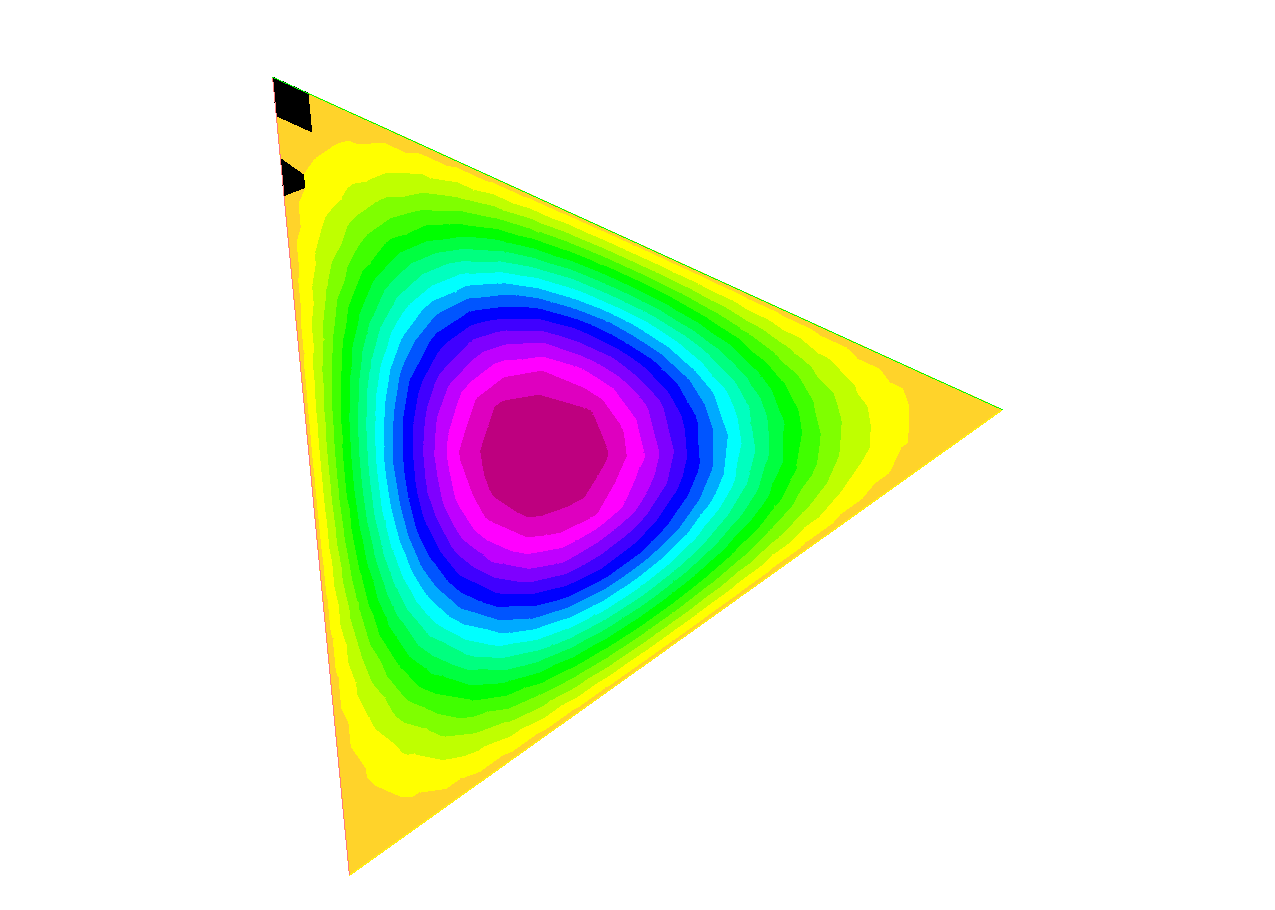
\includegraphics[width=0.33\textwidth]{3sides}
    }
    \subfloat[Caption 2]{
        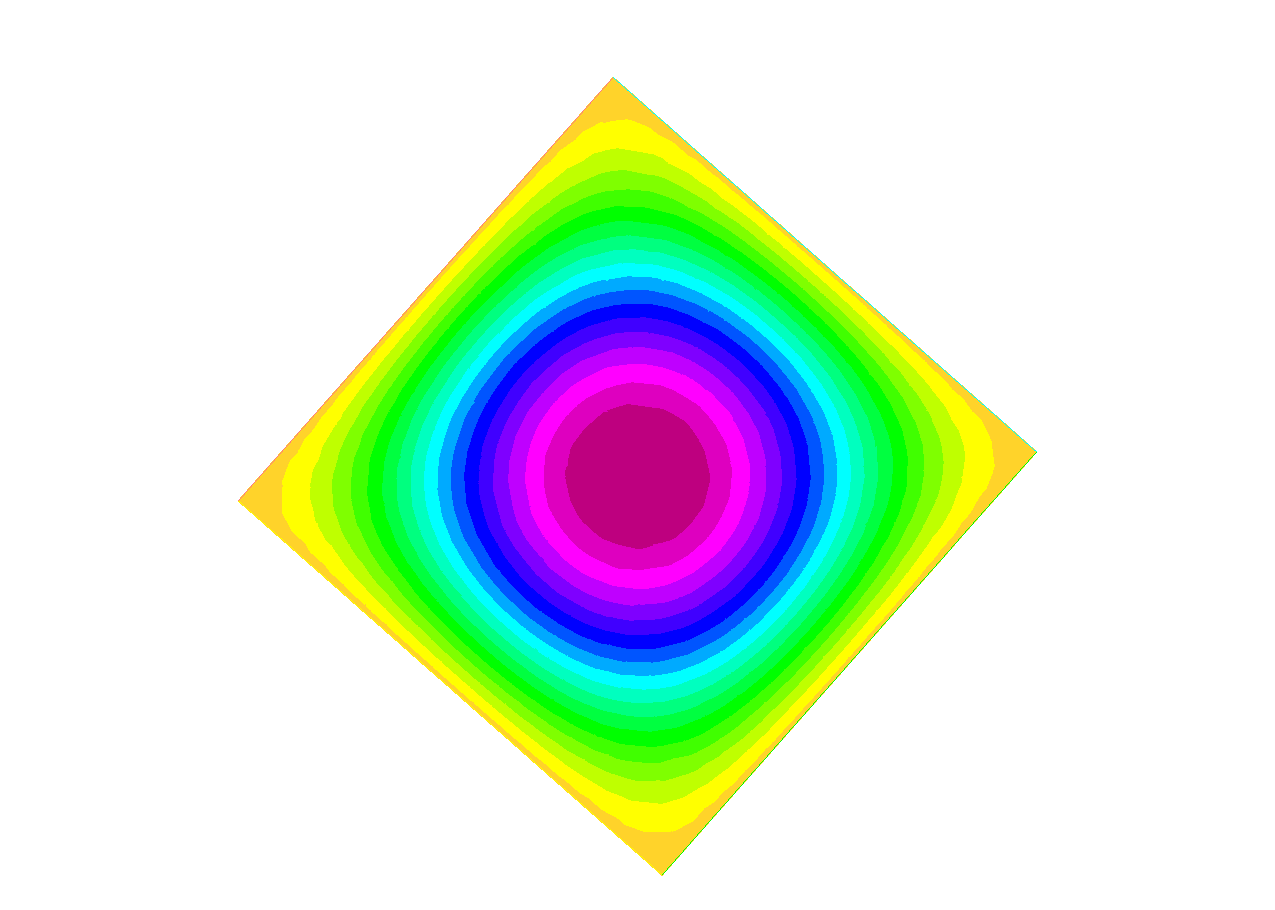
\includegraphics[width=0.33\textwidth]{4sides}
    }
    \subfloat[Caption y]{
        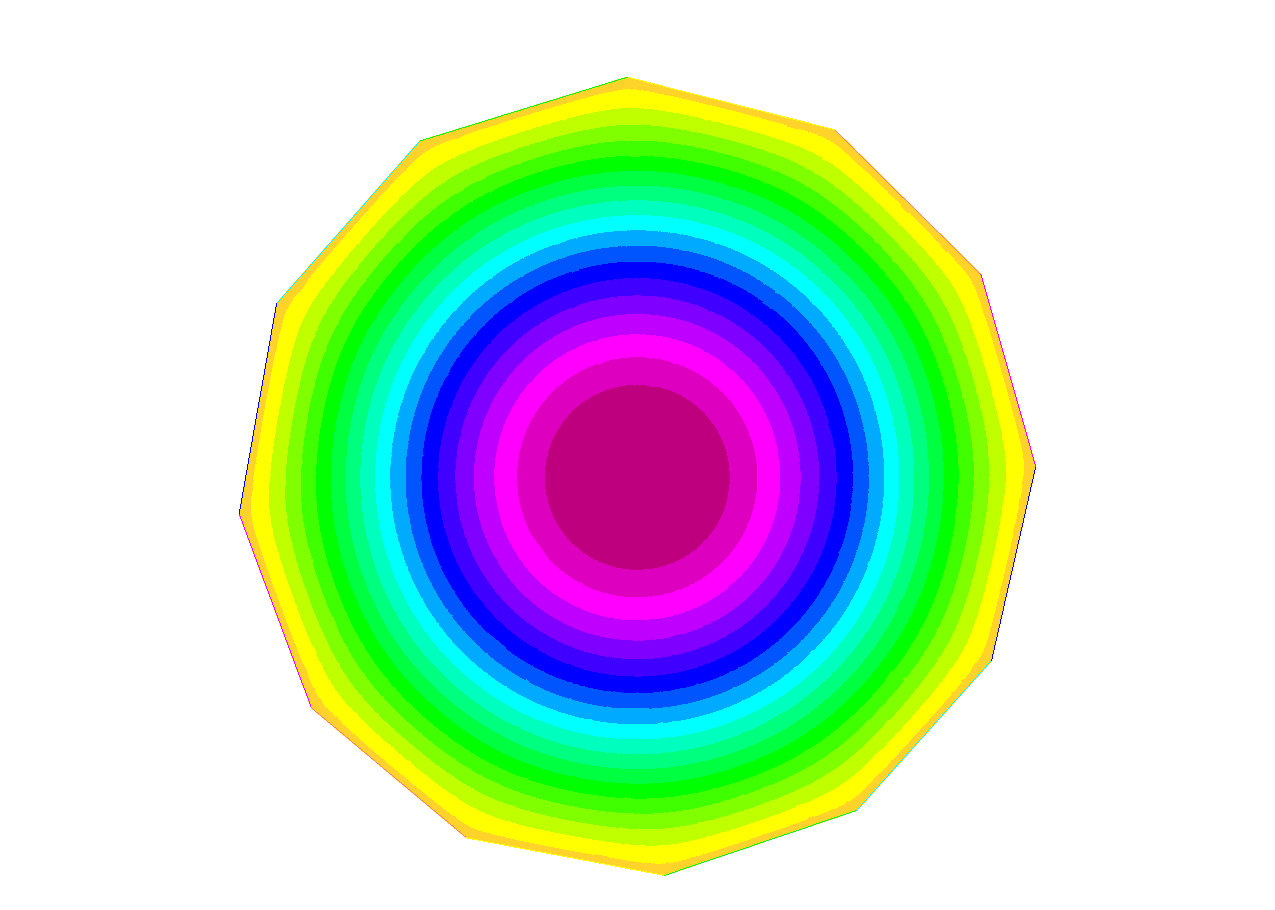
\includegraphics[width=0.33\textwidth]{12sides}
    }

    \subfloat[$N = 3$]{
        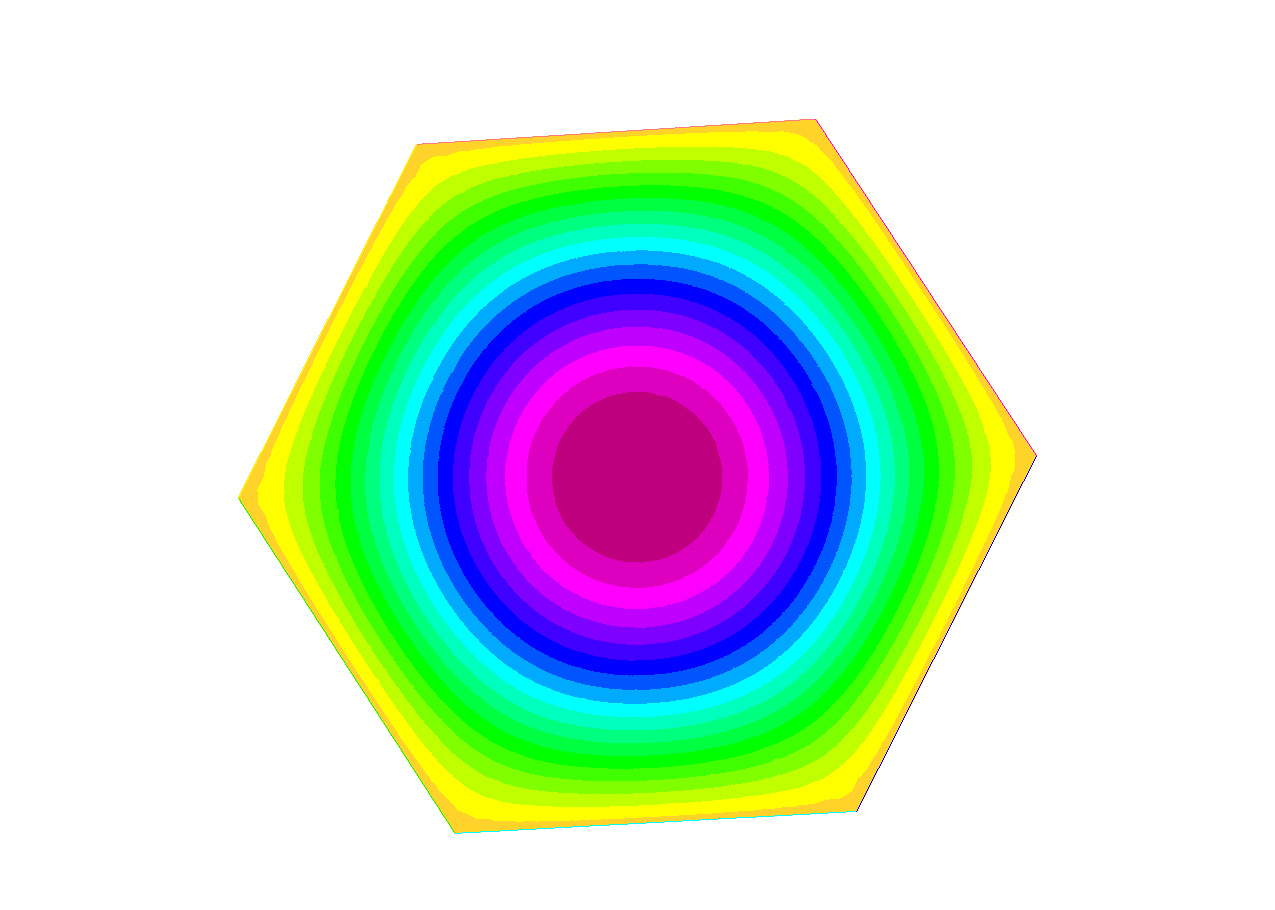
\includegraphics[width=0.5\textwidth]{6sides}
    }
    \subfloat[Caption 4]{
        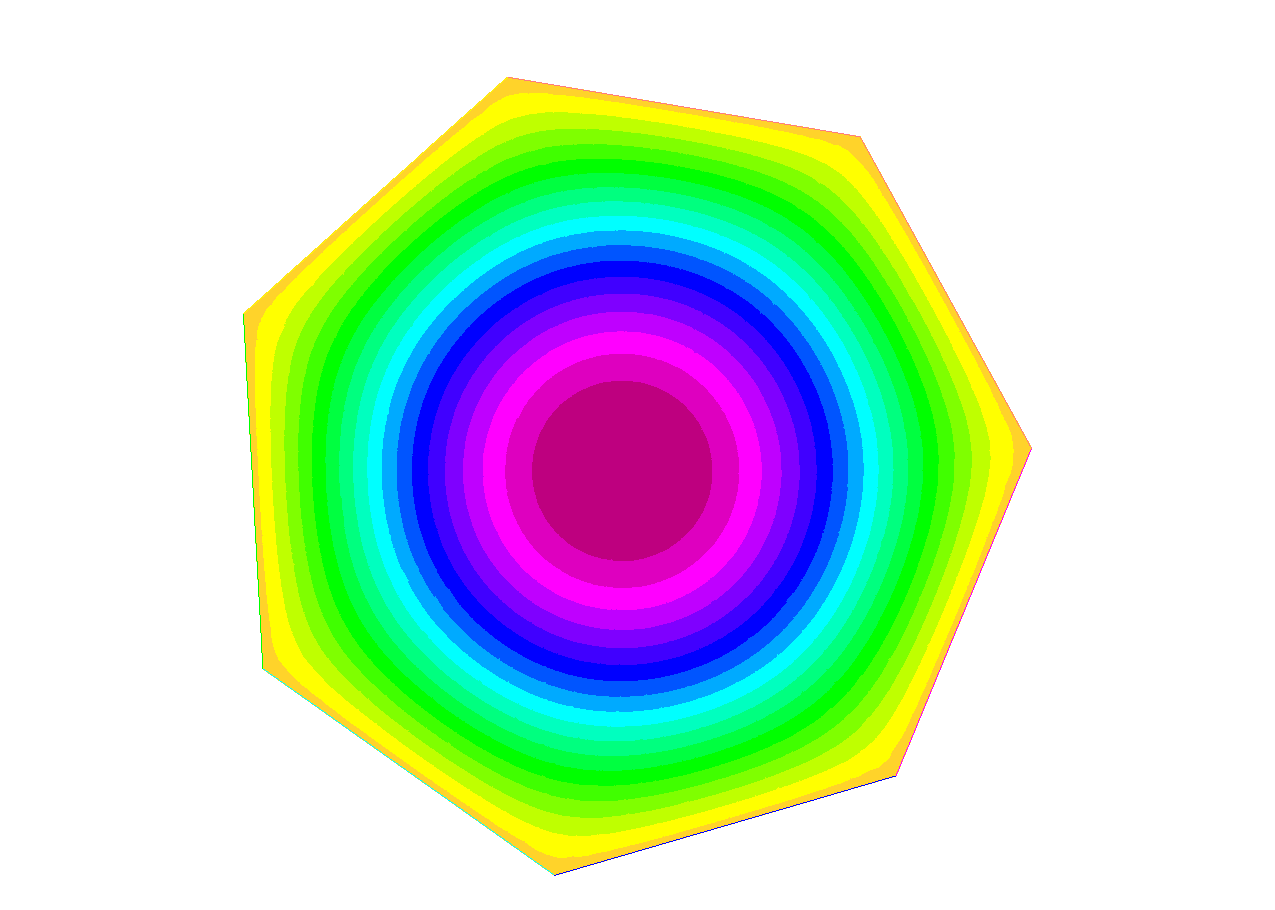
\includegraphics[width=0.5\textwidth]{7sides}
    }

    \caption{Overall caption}
\end{figure}

\break
 



\appendix
\chapter{Numerical Results}
\break

All of the figures are from the code written as a companion to this thesis (see \cite{code}).
The details needed to reproduce the program and the results are given in the repository.
Namely, we list the operating system, programming language, external libraries, and visualization software used.


  
\todo[inline]{Use table 5.1 in bogosel (page 173) as inspiration for our tables}



\todo[inline]{Table: min problem without constraint, num edges, stds, max diff of sides, product we are minimizing}
\begin{table}[h!]
  \centering
  \begin{tabular}{ c  c  c  c  c  }
    \toprule
    \makecell{$| P |$} & min value & diff of sides & SD Edges & SD Angles  \\ [0.5ex]
    \midrule
      3  & z & z & $2e-4$ & $1e-4$ \\
      4  & z & z & $3e-4$ & $6e-4$ \\
      5  & z & z & $7e-4$ & $2e-4$ \\
      6  & z & z & $8e-3$ & $5e-3$ \\
      7  & z & z & $3e-3$ & $2e-3$ \\
      8  & z & z & $1e-3$ & $3e-4$ \\
      9  & z & z & $7e-3$ & $6e-3$ \\
      10 & z & z & $5e-4$ & $7e-4$ \\
      11 & z & z & $1e-2$ & $6e-3$ \\
      12 & z & z & $2e-2$ & $1e-2$ \\
    f & i & n & a & l \\ [1ex]
    \bottomrule
  \end{tabular}
\end{table}


\begin{table}[hbt!]
  \begin{minipage}{.5\linewidth}
    \centering
    \begin{tabular}{ *{3}{c} }
      \toprule
      \makecell{$| P |$} & \makecell{$\sigma_{E}$} & \makecell{$\sigma_{A}$} \\
      \midrule
      3  & $2e-4$ & $1e-4$ \\
      4  & $3e-4$ & $6e-4$ \\
      5  & $7e-4$ & $2e-4$ \\
      6  & $8e-3$ & $5e-3$ \\
      7  & $3e-3$ & $2e-3$ \\
      8  & $1e-3$ & $3e-4$ \\
      9  & $7e-3$ & $6e-3$ \\
      10 & $5e-4$ & $7e-4$ \\
      11 & $1e-2$ & $6e-3$ \\
      12 & $2e-2$ & $1e-2$ \\
       &  &  \\
      \bottomrule
    \end{tabular}
    % \caption{HRV Dataset}\label{tab:first}
  \end{minipage}%
  \begin{minipage}{.5\linewidth}
    \centering
    \begin{tabular}{ *{3}{c} }
      \toprule
      \makecell{$| P |$} & \makecell{$\sigma_{E}$} & \makecell{$\sigma_{A}$} \\
      \midrule
      13 & $2e-2$ & $1e-2$ \\
      14 & $1e-2$ & $8e-3$ \\
      15 & $1e-2$ & $1e-2$ \\
      16 & $1e-2$ & $1e-2$ \\
      17 & $2e-2$ & $2e-2$ \\
      18 & $2e-2$ & $1e-2$ \\
      19 & $7e-3$ & $1e-2$ \\
      20 & $1e-2$ & $2e-2$ \\
      21 & $1e-2$ & $2e-2$ \\
      22 & $2e-2$ & $1e-2$ \\
      23 & $2e-2$ & $2e-2$ \\
      \bottomrule
    \end{tabular}
  \end{minipage}
  % \caption{The standard deviations of side lengths and angles}
\end{table}



\todo[inline]{Table: array of polygon figures alongside the number of vertices and its eigenvalue for fixed area=1}

\break
 
\printbibliography
 
\end{document}
